% Options for packages loaded elsewhere
% Options for packages loaded elsewhere
\PassOptionsToPackage{unicode}{hyperref}
\PassOptionsToPackage{hyphens}{url}
\PassOptionsToPackage{dvipsnames,svgnames,x11names}{xcolor}
%
\documentclass[
  letterpaper,
  DIV=11,
  numbers=noendperiod]{scrartcl}
\usepackage{xcolor}
\usepackage{amsmath,amssymb}
\setcounter{secnumdepth}{-\maxdimen} % remove section numbering
\usepackage{iftex}
\ifPDFTeX
  \usepackage[T1]{fontenc}
  \usepackage[utf8]{inputenc}
  \usepackage{textcomp} % provide euro and other symbols
\else % if luatex or xetex
  \usepackage{unicode-math} % this also loads fontspec
  \defaultfontfeatures{Scale=MatchLowercase}
  \defaultfontfeatures[\rmfamily]{Ligatures=TeX,Scale=1}
\fi
\usepackage{lmodern}
\ifPDFTeX\else
  % xetex/luatex font selection
\fi
% Use upquote if available, for straight quotes in verbatim environments
\IfFileExists{upquote.sty}{\usepackage{upquote}}{}
\IfFileExists{microtype.sty}{% use microtype if available
  \usepackage[]{microtype}
  \UseMicrotypeSet[protrusion]{basicmath} % disable protrusion for tt fonts
}{}
\makeatletter
\@ifundefined{KOMAClassName}{% if non-KOMA class
  \IfFileExists{parskip.sty}{%
    \usepackage{parskip}
  }{% else
    \setlength{\parindent}{0pt}
    \setlength{\parskip}{6pt plus 2pt minus 1pt}}
}{% if KOMA class
  \KOMAoptions{parskip=half}}
\makeatother
% Make \paragraph and \subparagraph free-standing
\makeatletter
\ifx\paragraph\undefined\else
  \let\oldparagraph\paragraph
  \renewcommand{\paragraph}{
    \@ifstar
      \xxxParagraphStar
      \xxxParagraphNoStar
  }
  \newcommand{\xxxParagraphStar}[1]{\oldparagraph*{#1}\mbox{}}
  \newcommand{\xxxParagraphNoStar}[1]{\oldparagraph{#1}\mbox{}}
\fi
\ifx\subparagraph\undefined\else
  \let\oldsubparagraph\subparagraph
  \renewcommand{\subparagraph}{
    \@ifstar
      \xxxSubParagraphStar
      \xxxSubParagraphNoStar
  }
  \newcommand{\xxxSubParagraphStar}[1]{\oldsubparagraph*{#1}\mbox{}}
  \newcommand{\xxxSubParagraphNoStar}[1]{\oldsubparagraph{#1}\mbox{}}
\fi
\makeatother

\usepackage{color}
\usepackage{fancyvrb}
\newcommand{\VerbBar}{|}
\newcommand{\VERB}{\Verb[commandchars=\\\{\}]}
\DefineVerbatimEnvironment{Highlighting}{Verbatim}{commandchars=\\\{\}}
% Add ',fontsize=\small' for more characters per line
\usepackage{framed}
\definecolor{shadecolor}{RGB}{241,243,245}
\newenvironment{Shaded}{\begin{snugshade}}{\end{snugshade}}
\newcommand{\AlertTok}[1]{\textcolor[rgb]{0.68,0.00,0.00}{#1}}
\newcommand{\AnnotationTok}[1]{\textcolor[rgb]{0.37,0.37,0.37}{#1}}
\newcommand{\AttributeTok}[1]{\textcolor[rgb]{0.40,0.45,0.13}{#1}}
\newcommand{\BaseNTok}[1]{\textcolor[rgb]{0.68,0.00,0.00}{#1}}
\newcommand{\BuiltInTok}[1]{\textcolor[rgb]{0.00,0.23,0.31}{#1}}
\newcommand{\CharTok}[1]{\textcolor[rgb]{0.13,0.47,0.30}{#1}}
\newcommand{\CommentTok}[1]{\textcolor[rgb]{0.37,0.37,0.37}{#1}}
\newcommand{\CommentVarTok}[1]{\textcolor[rgb]{0.37,0.37,0.37}{\textit{#1}}}
\newcommand{\ConstantTok}[1]{\textcolor[rgb]{0.56,0.35,0.01}{#1}}
\newcommand{\ControlFlowTok}[1]{\textcolor[rgb]{0.00,0.23,0.31}{\textbf{#1}}}
\newcommand{\DataTypeTok}[1]{\textcolor[rgb]{0.68,0.00,0.00}{#1}}
\newcommand{\DecValTok}[1]{\textcolor[rgb]{0.68,0.00,0.00}{#1}}
\newcommand{\DocumentationTok}[1]{\textcolor[rgb]{0.37,0.37,0.37}{\textit{#1}}}
\newcommand{\ErrorTok}[1]{\textcolor[rgb]{0.68,0.00,0.00}{#1}}
\newcommand{\ExtensionTok}[1]{\textcolor[rgb]{0.00,0.23,0.31}{#1}}
\newcommand{\FloatTok}[1]{\textcolor[rgb]{0.68,0.00,0.00}{#1}}
\newcommand{\FunctionTok}[1]{\textcolor[rgb]{0.28,0.35,0.67}{#1}}
\newcommand{\ImportTok}[1]{\textcolor[rgb]{0.00,0.46,0.62}{#1}}
\newcommand{\InformationTok}[1]{\textcolor[rgb]{0.37,0.37,0.37}{#1}}
\newcommand{\KeywordTok}[1]{\textcolor[rgb]{0.00,0.23,0.31}{\textbf{#1}}}
\newcommand{\NormalTok}[1]{\textcolor[rgb]{0.00,0.23,0.31}{#1}}
\newcommand{\OperatorTok}[1]{\textcolor[rgb]{0.37,0.37,0.37}{#1}}
\newcommand{\OtherTok}[1]{\textcolor[rgb]{0.00,0.23,0.31}{#1}}
\newcommand{\PreprocessorTok}[1]{\textcolor[rgb]{0.68,0.00,0.00}{#1}}
\newcommand{\RegionMarkerTok}[1]{\textcolor[rgb]{0.00,0.23,0.31}{#1}}
\newcommand{\SpecialCharTok}[1]{\textcolor[rgb]{0.37,0.37,0.37}{#1}}
\newcommand{\SpecialStringTok}[1]{\textcolor[rgb]{0.13,0.47,0.30}{#1}}
\newcommand{\StringTok}[1]{\textcolor[rgb]{0.13,0.47,0.30}{#1}}
\newcommand{\VariableTok}[1]{\textcolor[rgb]{0.07,0.07,0.07}{#1}}
\newcommand{\VerbatimStringTok}[1]{\textcolor[rgb]{0.13,0.47,0.30}{#1}}
\newcommand{\WarningTok}[1]{\textcolor[rgb]{0.37,0.37,0.37}{\textit{#1}}}

\usepackage{longtable,booktabs,array}
\usepackage{calc} % for calculating minipage widths
% Correct order of tables after \paragraph or \subparagraph
\usepackage{etoolbox}
\makeatletter
\patchcmd\longtable{\par}{\if@noskipsec\mbox{}\fi\par}{}{}
\makeatother
% Allow footnotes in longtable head/foot
\IfFileExists{footnotehyper.sty}{\usepackage{footnotehyper}}{\usepackage{footnote}}
\makesavenoteenv{longtable}
\usepackage{graphicx}
\makeatletter
\newsavebox\pandoc@box
\newcommand*\pandocbounded[1]{% scales image to fit in text height/width
  \sbox\pandoc@box{#1}%
  \Gscale@div\@tempa{\textheight}{\dimexpr\ht\pandoc@box+\dp\pandoc@box\relax}%
  \Gscale@div\@tempb{\linewidth}{\wd\pandoc@box}%
  \ifdim\@tempb\p@<\@tempa\p@\let\@tempa\@tempb\fi% select the smaller of both
  \ifdim\@tempa\p@<\p@\scalebox{\@tempa}{\usebox\pandoc@box}%
  \else\usebox{\pandoc@box}%
  \fi%
}
% Set default figure placement to htbp
\def\fps@figure{htbp}
\makeatother





\setlength{\emergencystretch}{3em} % prevent overfull lines

\providecommand{\tightlist}{%
  \setlength{\itemsep}{0pt}\setlength{\parskip}{0pt}}



 


\KOMAoption{captions}{tableheading}
\makeatletter
\@ifpackageloaded{caption}{}{\usepackage{caption}}
\AtBeginDocument{%
\ifdefined\contentsname
  \renewcommand*\contentsname{Table of contents}
\else
  \newcommand\contentsname{Table of contents}
\fi
\ifdefined\listfigurename
  \renewcommand*\listfigurename{List of Figures}
\else
  \newcommand\listfigurename{List of Figures}
\fi
\ifdefined\listtablename
  \renewcommand*\listtablename{List of Tables}
\else
  \newcommand\listtablename{List of Tables}
\fi
\ifdefined\figurename
  \renewcommand*\figurename{Figure}
\else
  \newcommand\figurename{Figure}
\fi
\ifdefined\tablename
  \renewcommand*\tablename{Table}
\else
  \newcommand\tablename{Table}
\fi
}
\@ifpackageloaded{float}{}{\usepackage{float}}
\floatstyle{ruled}
\@ifundefined{c@chapter}{\newfloat{codelisting}{h}{lop}}{\newfloat{codelisting}{h}{lop}[chapter]}
\floatname{codelisting}{Listing}
\newcommand*\listoflistings{\listof{codelisting}{List of Listings}}
\makeatother
\makeatletter
\makeatother
\makeatletter
\@ifpackageloaded{caption}{}{\usepackage{caption}}
\@ifpackageloaded{subcaption}{}{\usepackage{subcaption}}
\makeatother
\usepackage{bookmark}
\IfFileExists{xurl.sty}{\usepackage{xurl}}{} % add URL line breaks if available
\urlstyle{same}
\hypersetup{
  pdftitle={Guide to Creating Combined Local-Level Geographic Datasets},
  colorlinks=true,
  linkcolor={blue},
  filecolor={Maroon},
  citecolor={Blue},
  urlcolor={Blue},
  pdfcreator={LaTeX via pandoc}}


\title{Guide to Creating Combined Local-Level Geographic Datasets}
\author{}
\date{}
\begin{document}
\maketitle


\section{Guide to Creating Combined Local-Level Geographic
Datasets}\label{guide-to-creating-combined-local-level-geographic-datasets}

\subsection{The Sub-County Data Gap in Local Government Policy
Analysis}\label{the-sub-county-data-gap-in-local-government-policy-analysis}

Local government policy analysts and decision makers face a critical
challenge in accessing granular, policy-relevant data at the sub-county
level. While county-level data has become increasingly available and
standardized across the United States, the lack of systematic collection
and dissemination of sub-county information creates significant
limitations for municipal and local government officials who need to
make informed decisions for their communities{[}1{]}{[}2{]}.

The fundamental issue lies in the fact that most public health and
demographic surveillance data are ``limited mostly to the county or
state level,'' creating a void where local decision makers need the most
granular information{[}2{]}. This data gap is particularly problematic
because local governments operate at a scale where county-level
aggregated data often obscures critical variations in community needs,
demographics, and outcomes that exist within county boundaries. For
instance, a county may show adequate performance on aggregate measures
while specific neighborhoods or sub-county areas experience significant
challenges that require targeted policy interventions{[}3{]}.

The shortage of sub-county data presents multiple barriers to effective
local governance. Most critically, it hampers the ability of local
officials to identify health disparities, infrastructure needs, and
social inequities within their jurisdictions that may be masked by
county-level aggregations{[}3{]}. This limitation is compounded by
technical challenges inherent in small-area data collection, including
``data and statistical reliability issues when using small case
(numerator) and population (denominator) numbers'' and confidentiality
concerns where individual identification might be possible in areas with
small populations{[}4{]}. These methodological constraints have led to
systematic underinvestment in sub-county data infrastructure, creating a
vicious cycle where the lack of reliable small-area data discourages
further development of collection and analysis capabilities.

Furthermore, the absence of standardized sub-county data collection
processes across different jurisdictions makes it difficult for local
governments to benchmark their performance, share best practices, or
coordinate regional responses to shared challenges{[}1{]}. While
initiatives like the CDC's Environmental Public Health Tracking Program
have begun developing methodologies for aggregating census tracts to
create more reliable sub-county geographies, these efforts remain
limited in scope and do not address the full range of policy-relevant
indicators that local decision makers require{[}4{]}. The result is that
local government policy analysts often must make critical decisions
about resource allocation, service delivery, and community development
without access to the granular, locally-relevant data that would enable
more targeted and effective interventions{[}5{]}{[}6{]}.

\subsection{The Need for Purpose-Built Sub-County
Datasets}\label{the-need-for-purpose-built-sub-county-datasets}

The data collection challenges outlined above ultimately point to a more
fundamental need: the construction of sub-county datasets that align
with the geographies that matter most to local decision makers, rather
than defaulting to existing statistical boundaries that may not reflect
the functional reality of how communities operate, how services are
delivered, or how policy interventions need to be targeted.

Local government officials require data for geographies that correspond
to their actual spheres of influence and responsibility. This includes
\textbf{neighborhoods} defined by social cohesion, economic activity,
and shared infrastructure rather than arbitrary census tract
boundaries{[}43{]}. It encompasses \textbf{metro corridors} where
transit-oriented development policies need implementation{[}44{]},
commercial districts where economic development strategies are focused,
school catchment areas where educational interventions are planned, and
service delivery zones where public health programs are deployed. These
functional areas rarely align with the neat administrative boundaries of
census tracts, ZIP codes, or county subdivisions that currently serve as
the default units for most data collection efforts{[}45{]}{[}46{]}.

The imperative for purpose-built datasets becomes particularly acute
when considering that many of the most pressing local policy challenges
operate across multiple traditional boundary systems. For instance,
addressing transportation equity requires understanding commuting
patterns that span multiple census tracts and ZIP codes{[}47{]}.
Tackling neighborhood-level health disparities requires data aggregation
that reflects actual community boundaries rather than statistical
convenience{[}48{]}. Economic development initiatives often need to
target specific commercial corridors or industrial zones that bear no
relationship to census geography{[}49{]}.

\subsection{The Challenge of Misaligned Geographic
Boundaries}\label{the-challenge-of-misaligned-geographic-boundaries}

Local government policy analysts frequently encounter a fundamental
challenge when working with geospatial data: datasets are often
aggregated at different geographic scales that do not align with each
other or with the specific geographic units of policy interest. This
misalignment creates what geographers call the ``Modifiable Areal Unit
Problem'' (MAUP), where the boundaries used for data collection may not
correspond to the boundaries that are most meaningful for policy
analysis or community engagement{[}82{]}.

Consider a scenario where a local government wants to understand how
internet connectivity (broadband speeds) relates to socioeconomic
conditions (median household income) within the context of
neighborhood-level civic engagement and representation. Such an analysis
is particularly relevant for Arlington County, Virginia, where 62
distinct civic associations serve as important channels for community
input and local governance{[}83{]}{[}84{]}. These civic associations
represent genuine neighborhood identities and community interests that
cross-cut the administrative boundaries used by federal agencies for
data collection and reporting.

\begin{figure}[H]

{\centering \pandocbounded{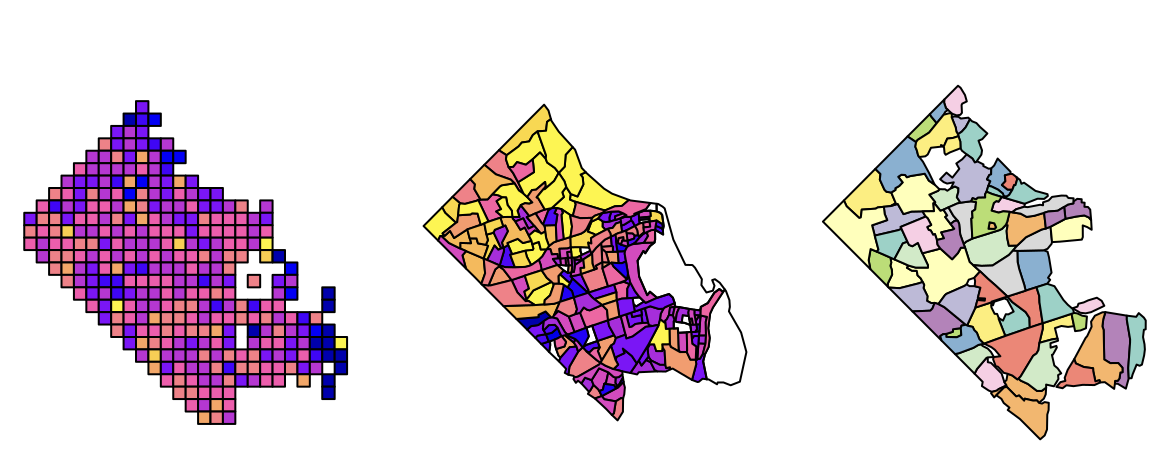
\includegraphics[keepaspectratio]{images/3plots.png}}

}

\caption{The goal is to transform both Ookla Broadband Speed data (left)
and American Community Survey Household Income data (center) into
Arlington County Civic Association geographies (right)}

\end{figure}%

The challenge becomes apparent when we consider the geographic scales at
which different types of data are available:

\textbf{Broadband Speed Data}: Companies like Ookla collect internet
speed test data and aggregate it into standardized tiles that are
approximately 610.8 meters by 610.8 meters (about 0.37 square
kilometers) at the equator{[}85{]}{[}86{]}{[}87{]}. These tiles are
created using a Web Mercator projection at zoom level 16 and are
designed to create manageable datasets from hundreds of millions of
speed tests taken monthly{[}88{]}. While this provides fine-scale
geographic detail, the tile boundaries bear no relationship to political
or community boundaries.

\textbf{Socioeconomic Data}: The U.S. Census Bureau's American Community
Survey (ACS) provides detailed demographic and economic data, including
median household income (variable B19013\_001), aggregated to census
geographic units such as census tracts and block groups{[}89{]}{[}90{]}.
The 5-year ACS estimates are available down to the census block group
level, which typically contain 600 to 3,000 people{[}89{]}. However,
these boundaries are designed for statistical efficiency rather than
community representation.

\textbf{Community Representation}: Arlington's civic associations
represent genuine neighborhood communities and serve as formal channels
for community input to local government{[}84{]}{[}91{]}. These
associations have boundaries that reflect actual community identities,
local landmarks, and neighborhood characteristics, but they do not align
with either Ookla tiles or census geography.

This misalignment creates several analytical challenges:

\begin{enumerate}
\def\labelenumi{\arabic{enumi}.}
\tightlist
\item
  \textbf{Ecological Fallacy}: Conclusions drawn from data aggregated at
  one geographic scale may not hold true at another scale
\item
  \textbf{Boundary Effects}: Important variations that occur near
  boundaries may be obscured or misrepresented
\item
  \textbf{Policy Relevance}: Analysis conducted at inappropriate
  geographic scales may not inform the actual decision-making units that
  matter for policy implementation
\end{enumerate}

\subsection{Why This Analysis Matters: Understanding the Digital Divide
at the Community
Level}\label{why-this-analysis-matters-understanding-the-digital-divide-at-the-community-level}

The relationship between internet access and socioeconomic status has
become a critical policy issue, particularly in the wake of the COVID-19
pandemic, which highlighted how digital connectivity affects access to
employment, education, healthcare, and civic
participation{[}92{]}{[}93{]}. Research has consistently shown that
broadband access is not equally distributed across communities, with
significant disparities based on income, race, ethnicity, and
geography{[}94{]}{[}95{]}.

Understanding these disparities at the neighborhood level is essential
for several reasons:

\textbf{Targeted Policy Interventions}: Effective broadband policy
requires understanding where the need is greatest and which communities
are underserved. Analysis at the civic association level can help
identify specific neighborhoods where public investments or policy
interventions would have the greatest impact{[}93{]}{[}96{]}.

\textbf{Community Engagement}: Civic associations serve as important
channels for community input and local governance. Understanding
broadband access patterns within these community-defined boundaries
enables more effective engagement with residents and community
leaders{[}91{]}.

\textbf{Equity Assessment}: Federal and local policies increasingly
emphasize digital equity as a civil rights issue{[}96{]}. Analysis at
the community level can help identify whether public investments and
policies are reaching the communities that need them most.

\textbf{Economic Development}: Research suggests that broadband access
can significantly impact household income, with some studies indicating
that upgrading from basic to high-speed broadband can increase household
income by thousands of dollars annually{[}97{]}. Understanding these
patterns at the neighborhood level can inform economic development
strategies.

\subsection{Data Description}\label{data-description}

\subsubsection{Ookla Speedtest Data}\label{ookla-speedtest-data}

Ookla's open dataset provides global fixed broadband and mobile network
performance metrics aggregated into Web Mercator tiles{[}85{]}{[}86{]}.
Key characteristics include:

\begin{itemize}
\tightlist
\item
  \textbf{Geographic Unit}: Zoom level 16 Web Mercator tiles
  (approximately 610.8m × 610.8m at the equator)
\item
  \textbf{Variables}: Average download speed, upload speed, and latency
  for each tile
\item
  \textbf{Data Source}: Aggregated from millions of speed tests taken
  via Speedtest applications
\item
  \textbf{Quality Control}: Measurements filtered to include only
  results with GPS-quality location accuracy
\item
  \textbf{Temporal Coverage}: Data available quarterly from 2019 onwards
\item
  \textbf{Projection}: EPSG:4326 (WGS 84) for geometric representation
\end{itemize}

{[}Map Insert Location 2: A detailed map showing Ookla tiles overlaid on
a portion of Arlington County, demonstrating the fine-scale grid pattern
and how it relates to local geography{]}

\subsubsection{American Community Survey
Data}\label{american-community-survey-data}

The ACS provides comprehensive demographic and economic data for the
United States{[}89{]}{[}90{]}. For this analysis, we focus on:

\begin{itemize}
\tightlist
\item
  \textbf{Variable}: B19013\_001 (Median Household Income in the past 12
  months)
\item
  \textbf{Geographic Unit}: Census block groups
\item
  \textbf{Dataset}: 5-year estimates (providing the finest geographic
  detail available)
\item
  \textbf{Sample}: Based on approximately 3.5 million addresses surveyed
  annually
\item
  \textbf{Margin of Error}: All estimates include margins of error
  reflecting sampling variability
\item
  \textbf{Currency}: Income figures are inflation-adjusted to current
  dollars
\end{itemize}

\subsubsection{Arlington Civic
Associations}\label{arlington-civic-associations}

Arlington County recognizes 62 civic associations that serve as formal
channels for community input and neighborhood
representation{[}98{]}{[}84{]}. These associations:

\begin{itemize}
\tightlist
\item
  \textbf{Boundaries}: Defined by community identity, local landmarks,
  and neighborhood characteristics
\item
  \textbf{Governance}: Each association elects representatives to the
  Arlington County Civic Federation
\item
  \textbf{Policy Role}: Provide formal input on development projects,
  transportation plans, and other local issues
\item
  \textbf{Geographic Coverage}: Comprehensive coverage of Arlington
  County's residential areas
\end{itemize}

{[}Map Insert Location 3: A comprehensive map of all 62 Arlington civic
associations with labels, showing the diversity in size and shape of
these community-defined boundaries{]}

\subsection{Methodological Approach}\label{methodological-approach}

\subsubsection{Census Data Disaggregation
Strategy}\label{census-data-disaggregation-strategy}

The approach for ACS data involves a two-step process:

\begin{enumerate}
\def\labelenumi{\arabic{enumi}.}
\item
  \textbf{Block Group to Block Disaggregation}: First, we distribute the
  block group-level median household income data evenly across all
  census blocks within each block group. This assumes that income is
  uniformly distributed within block groups, which is a simplifying
  assumption but necessary given data availability
  constraints{[}82{]}{[}104{]}.
\item
  \textbf{Block to Civic Association Aggregation}: Second, we aggregate
  the block-level estimates up to civic association boundaries using
  area-weighted methods. This preserves the total population and income
  estimates while respigning them to policy-relevant geographic
  units{[}105{]}.
\end{enumerate}

{[}Diagram Insert Location 1: A flowchart showing the data
transformation process from source geographies to target geography{]}

\pandocbounded{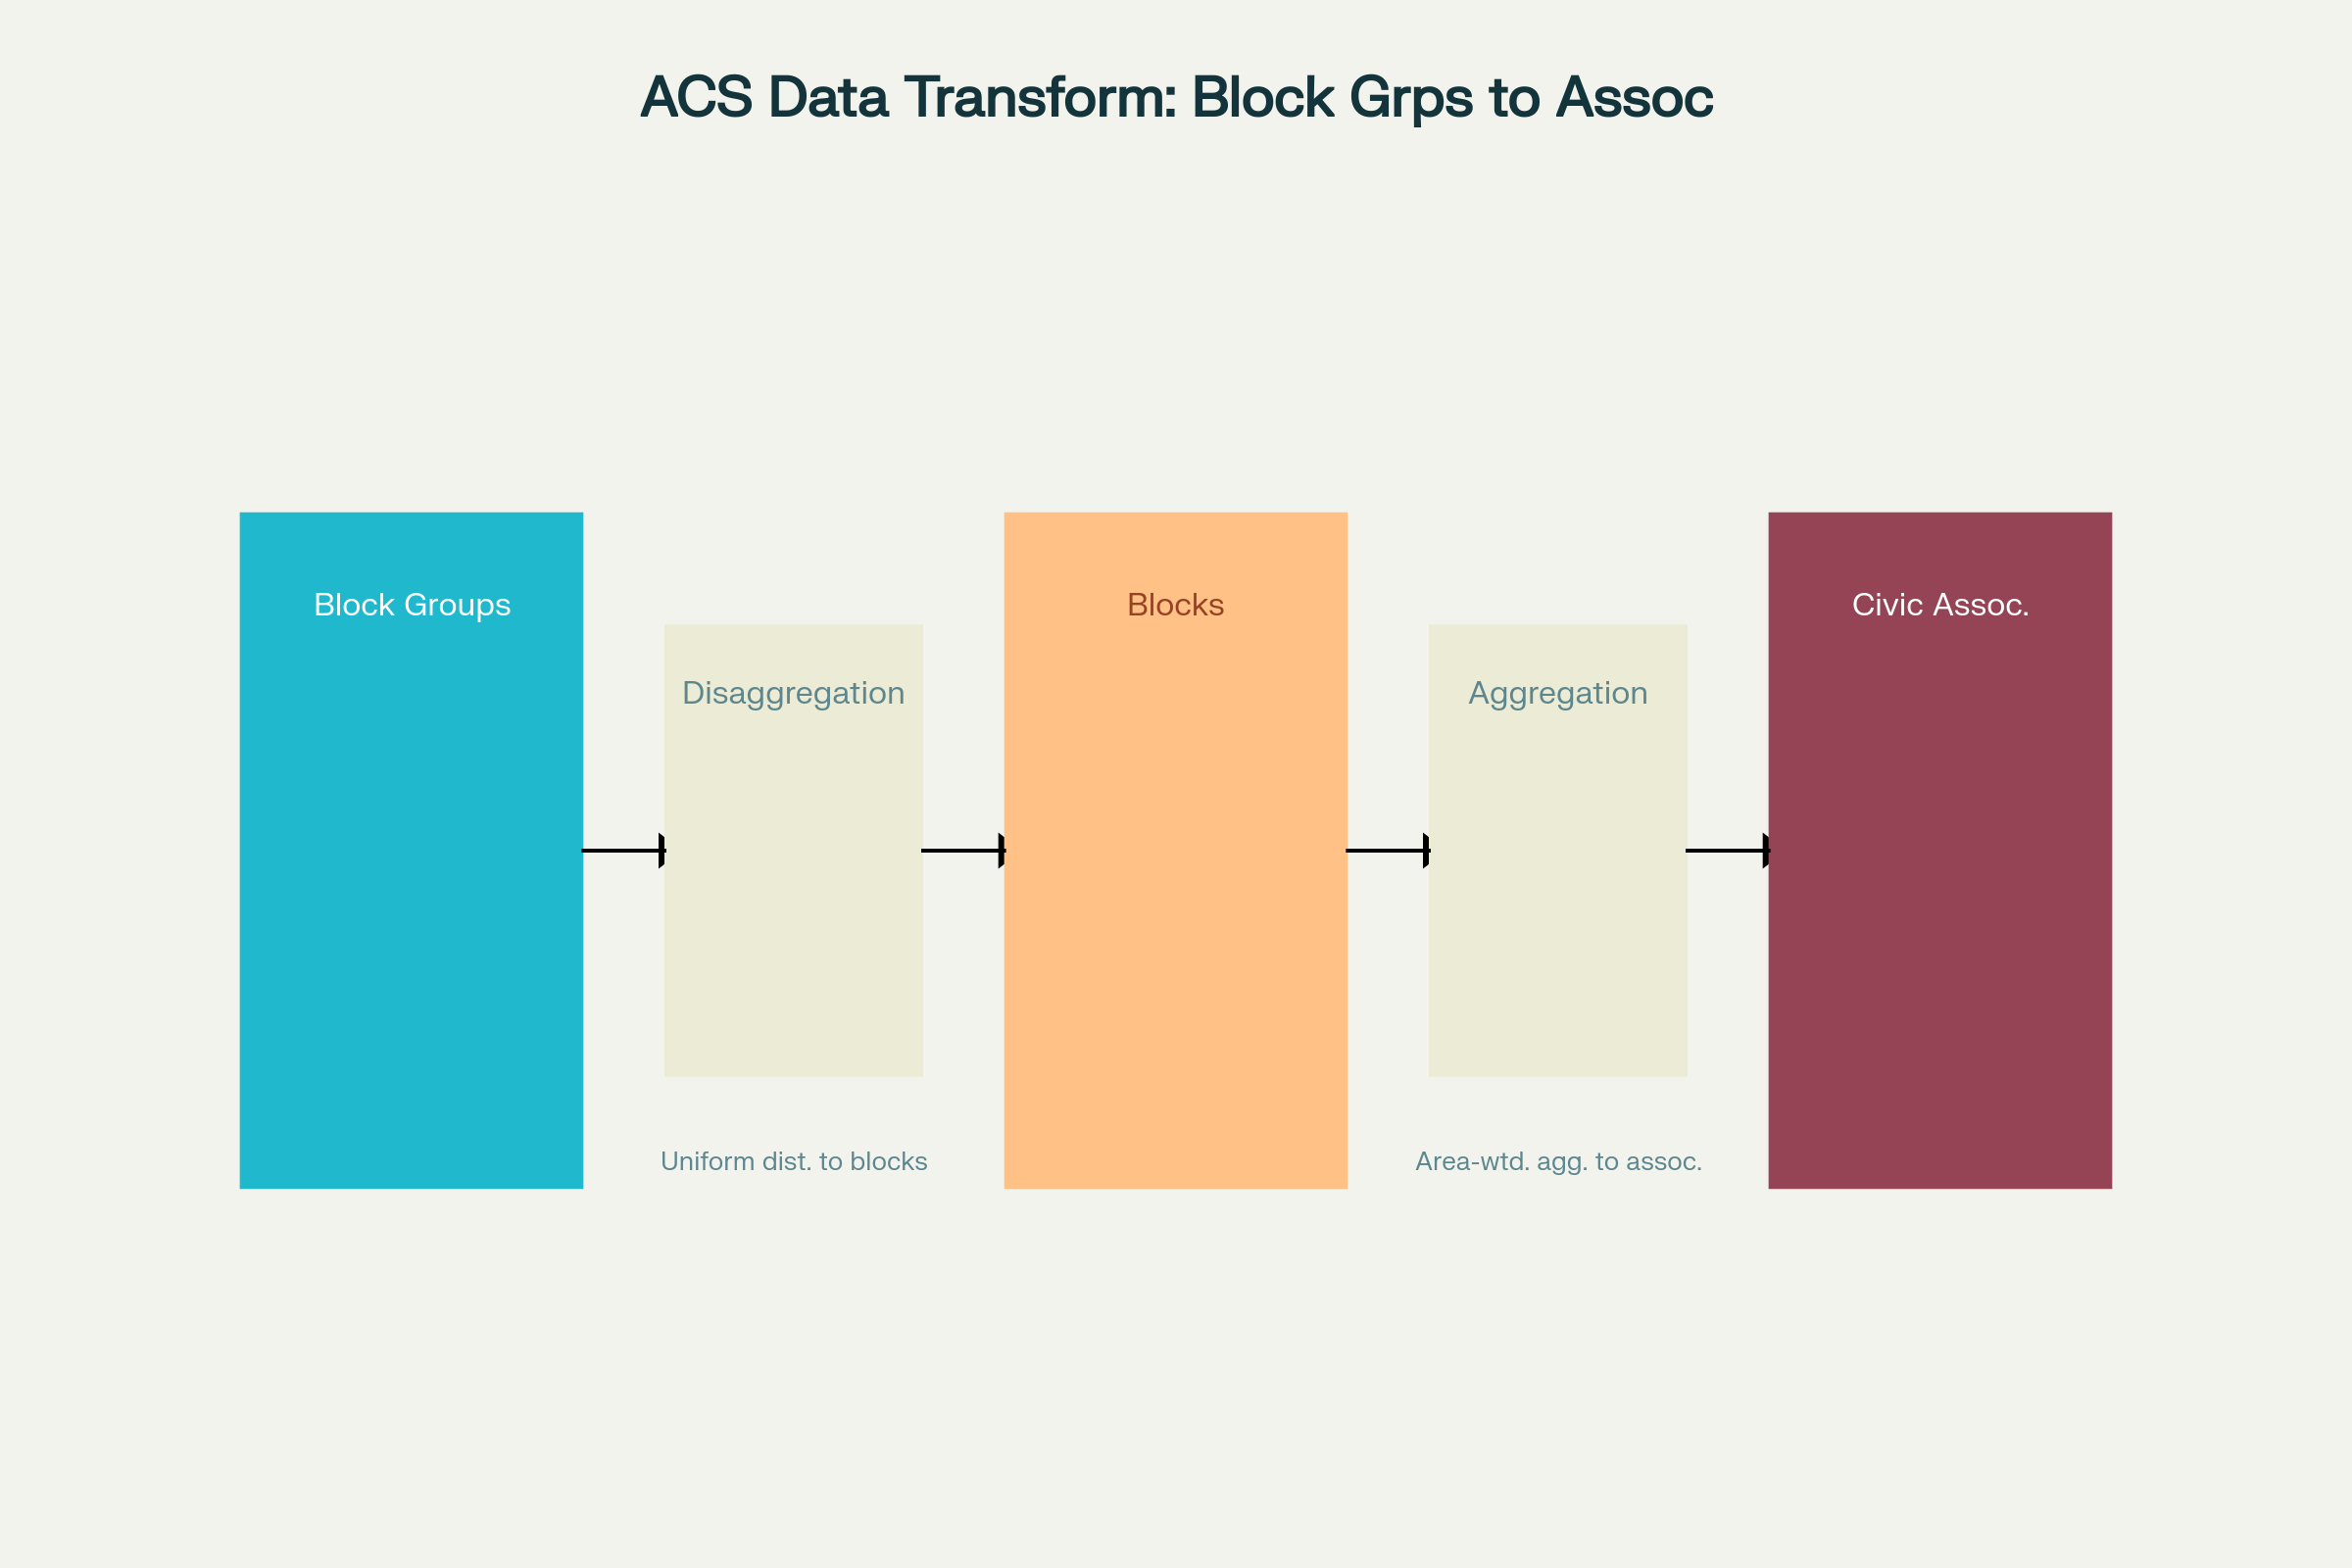
\includegraphics[keepaspectratio]{images/ACS Data Transform.png}}

This two-step approach is necessary because: - ACS data is not available
at the census block level for most variables - Census blocks provide a
finer geographic resolution that better supports accurate areal
interpolation - The hierarchical relationship between blocks and block
groups ensures data consistency

\subsubsection{Understanding Areal
Interpolation}\label{understanding-areal-interpolation}

Areal interpolation is a spatial analysis technique that estimates
values for one set of geographic areas (target zones) based on known
values from a different set of geographic areas (source zones) that
overlap but do not have coincident boundaries{[}99{]}{[}100{]}. This
technique is essential when combining datasets that use different
geographic reporting units.

The fundamental assumption underlying areal interpolation is that the
phenomenon being studied has some predictable spatial distribution
pattern. Different interpolation methods make different assumptions
about this distribution:

\textbf{Areal Weighted Interpolation}: Assumes that the variable of
interest is uniformly distributed within each source zone. Values are
allocated to target zones proportionally based on the area of
overlap{[}100{]}{[}101{]}.

\textbf{Dasymetric Mapping}: Uses additional data sources (such as land
use data) to refine the allocation, recognizing that variables like
population are not uniformly distributed across space{[}100{]}{[}102{]}.

\textbf{Pycnophylactic Interpolation}: Creates smooth surfaces that
avoid sharp discontinuities between adjacent areas while preserving the
total value from source zones{[}100{]}{[}103{]}.

For broadband speed data from Ookla tiles, areal weighted interpolation
is appropriate because the tiles are relatively small and uniform, and
the underlying assumption that internet speeds are relatively consistent
within each tile is reasonable{[}99{]}.

\pandocbounded{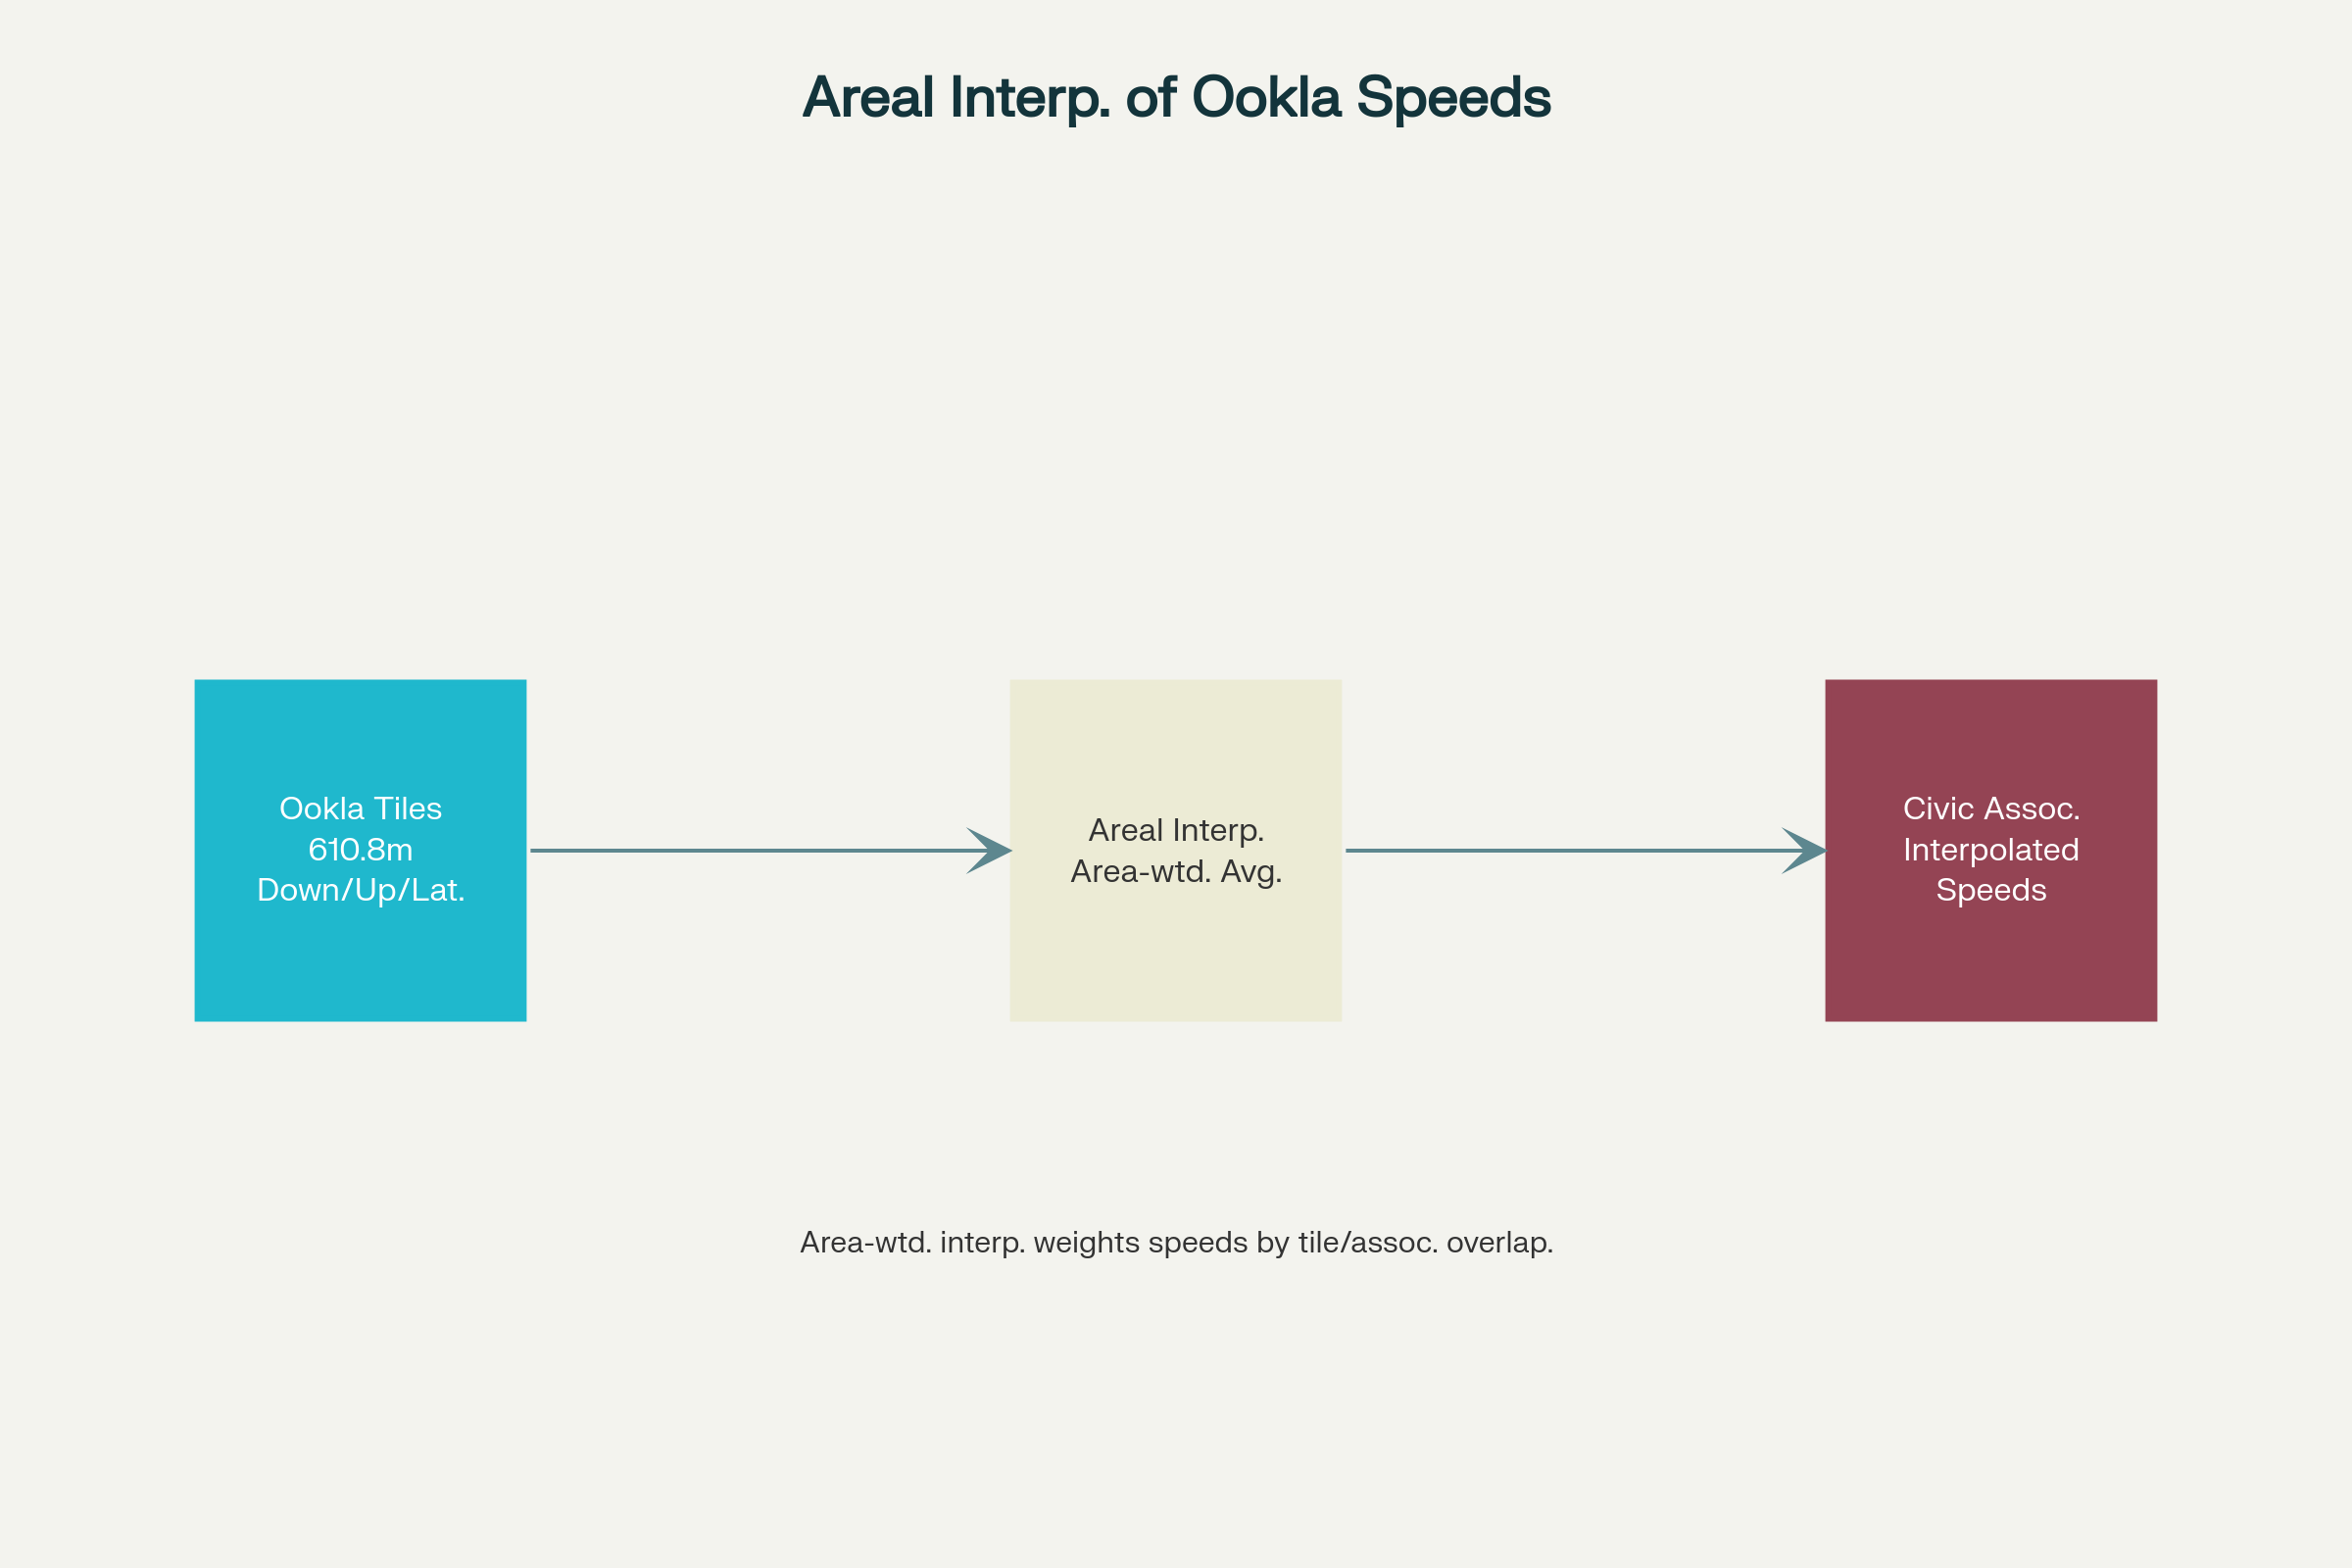
\includegraphics[keepaspectratio]{images/Ookla transform.png}}

\textbf{Single-Step Process}: Unlike the ACS data transformation which
required two steps (disaggregation then aggregation), the Ookla
broadband data transformation is a direct, single-step process using
areal interpolation.

\textbf{Source Data Characteristics}: - \textbf{Ookla Tiles}: Web
Mercator tiles at zoom level 16 (approximately 610.8m × 610.8m at the
equator) - \textbf{Data Variables}: Average download speed, upload
speed, latency, and number of tests per tile - \textbf{Coverage}:
Fine-scale geographic detail with standardized tile boundaries

\textbf{Areal Interpolation Methodology}: - \textbf{Area-Weighted
Averaging}: Speed values are weighted by the intersection area between
Ookla tiles and civic association boundaries - \textbf{Preservation of
Data Integrity}: The method maintains the statistical properties of the
original speed measurements while transforming to policy-relevant
boundaries - \textbf{Quality Control}: Tiles with insufficient test
samples (\textless{} 5 tests) are filtered out to ensure statistical
reliability

\textbf{Target Geography Benefits}: - \textbf{Policy Relevance}: Results
align with civic association boundaries that matter for community
engagement and local governance - \textbf{Community Scale}: Analysis
conducted at the neighborhood level where digital equity interventions
are most effective - \textbf{Direct Application}: Output can be
immediately used for infrastructure planning and resource allocation
decisions

This transformation enables Arlington County to understand broadband
performance patterns at the civic association level, supporting targeted
digital equity initiatives and evidence-based policy making for
community-specific infrastructure investments.

\subsubsection{Validation and
Uncertainty}\label{validation-and-uncertainty}

All areal interpolation methods introduce uncertainty, and it's
important to acknowledge and, where possible, quantify this uncertainty:

\textbf{Source Data Quality}: Both Ookla and ACS data have inherent
limitations. Ookla data may be biased toward areas with more active
internet users, while ACS data has sampling margins of error that
increase for smaller geographic areas{[}89{]}{[}106{]}.

\textbf{Interpolation Uncertainty}: The accuracy of areal interpolation
depends on how well the underlying assumptions match reality. Uniform
distribution assumptions may not hold in areas with significant
variation in population density or land use patterns{[}100{]}{[}101{]}.

\textbf{Boundary Effects}: Civic association boundaries may cross areas
with different characteristics, potentially leading to averaging effects
that obscure important local variations{[}82{]}.

\subsection{Step-by-Step Implementation
Process}\label{step-by-step-implementation-process}

\subsubsection{Step 1: Data Acquisition}\label{step-1-data-acquisition}

\textbf{Ookla Data}: 1. Download quarterly Ookla data from the GitHub
repository (https://github.com/teamookla/ookla-open-data) 2. Filter data
to Arlington County bounding box to reduce file size 3. Select most
recent available quarter for analysis 4. Choose either fixed broadband
or mobile data based on research question

\textbf{ACS Data}: 1. Use Census API or tidycensus package to download
block group-level data for Arlington County 2. Download median household
income (B19013\_001) with margin of error 3. Obtain both 2020 census
block and block group boundary files 4. Ensure all data uses the same
coordinate reference system

\textbf{Civic Association Boundaries}: 1. Load the provided GeoJSON file
containing Arlington civic association boundaries 2. Verify coordinate
reference system matches other datasets 3. Check for any gaps or
overlaps in coverage

\subsubsection{Step 2: Data
Preprocessing}\label{step-2-data-preprocessing}

\textbf{Coordinate System Standardization}:

\begin{verbatim}
# All datasets should be projected to the same coordinate system
# For local analysis, use a projected coordinate system like State Plane Virginia North
target_crs <- "EPSG:3968"  # State Plane Virginia North (US Feet)
\end{verbatim}

\textbf{Data Quality Checks}: 1. Verify that all civic associations are
represented 2. Check for missing data in ACS variables 3. Validate that
Ookla tiles have reasonable speed values 4. Ensure block group and block
geographies nest properly

\subsubsection{Step 3: Areal Interpolation
Implementation}\label{step-3-areal-interpolation-implementation}

\textbf{Ookla to Civic Associations}: 1. Calculate intersection areas
between Ookla tiles and civic association boundaries 2. Weight speed
values by intersection area 3. Aggregate weighted values to civic
association level 4. Calculate both area-weighted means and total area
coverage

\textbf{ACS Block Group to Block Disaggregation}: 1. Spatially join
blocks to their parent block groups 2. Assign block group median income
value to all blocks within the group 3. This assumes uniform income
distribution within block groups

\textbf{Block to Civic Association Aggregation}: 1. Calculate
intersection areas between census blocks and civic associations 2.
Weight population by intersection area 3. Calculate population-weighted
average income for each civic association 4. Preserve margins of error
through error propagation methods

{[}Code Block Insert Location 1: Example R code showing the areal
interpolation workflow{]}

\subsubsection{Step 4: Data Integration and
Validation}\label{step-4-data-integration-and-validation}

\textbf{Combine Datasets}: 1. Join interpolated broadband speeds with
interpolated income data by civic association 2. Calculate additional
variables such as speed categories or income quintiles 3. Create quality
indicators showing interpolation confidence

\textbf{Validation Steps}: 1. Check that total population matches source
data 2. Verify that interpolated values fall within reasonable ranges 3.
Compare results to known patterns or alternative data sources where
available 4. Calculate and report interpolation uncertainty estimates

\subsubsection{Step 5: Analysis and
Visualization}\label{step-5-analysis-and-visualization}

\textbf{Exploratory Analysis}: 1. Create choropleth maps showing speed
and income distributions 2. Calculate correlation coefficients between
speed and income 3. Identify outlier civic associations for further
investigation

\textbf{Statistical Analysis}: 1. Test for spatial autocorrelation in
both variables 2. Estimate regression models accounting for spatial
relationships 3. Control for potential confounding variables such as
population density

{[}Map Insert Location 5: A series of small multiple maps showing how
the analysis could be extended to other variables or time periods{]}

\section{Implementation of Arlington Broadband and Income Analysis Using
Complete
Datasets}\label{implementation-of-arlington-broadband-and-income-analysis-using-complete-datasets}

\subsection{Dataset Validation and
Preparation}\label{dataset-validation-and-preparation}

\subsubsection{Available Data
Assessment}\label{available-data-assessment}

\textbf{Census Blocks (va013\_geo\_blocks.geojson)}: The census block
dataset contains 2,431 individual blocks covering Arlington County, with
essential attributes including: - Population (POP20): Ranges from 0 to
688 residents per block - Housing units (HOUSING20): From 0 to 427 units
per block\\
- Land area (ALAND20): Highly variable, from small urban blocks to
larger areas - Geographic identifiers (GEOID20): Enabling linkage to ACS
data

\textbf{Civic Association Boundaries
(va013\_geo\_arl\_2021\_civic\_associations.geojson)}: Contains all 62
Arlington civic associations including: - Williamsburg, Old Dominion,
Maywood, Ballston-Virginia Square - Major associations like Bluemont,
Clarendon-Courthouse, Arlington Heights - Smaller neighborhoods like
Cherry Valley Nature Area and Rivercrest

\textbf{Spatial Coverage Analysis}: The civic associations provide
comprehensive coverage of Arlington County's residential areas, with
boundaries that reflect genuine community identities rather than
administrative convenience. Block sizes vary significantly, from dense
urban cores to larger suburban areas, which will affect interpolation
accuracy. \#\# Methodology Implementation

\subsubsection{Step 1: Coordinate System
Standardization}\label{step-1-coordinate-system-standardization}

R

\begin{Shaded}
\begin{Highlighting}[]
\CommentTok{\# Load required libraries}
\FunctionTok{library}\NormalTok{(sf)}
\FunctionTok{library}\NormalTok{(dplyr)}
\FunctionTok{library}\NormalTok{(areal)}

\CommentTok{\# Standardize all datasets to Virginia State Plane North}
\NormalTok{target\_crs }\OtherTok{\textless{}{-}} \StringTok{"EPSG:3968"}

\CommentTok{\# Load and transform datasets}
\NormalTok{civic\_associations }\OtherTok{\textless{}{-}}
  \FunctionTok{st\_read}\NormalTok{(}\StringTok{"va013\_geo\_arl\_2021\_civic\_associations.geojson"}\NormalTok{) }\SpecialCharTok{\%\textgreater{}\%}
  \FunctionTok{st\_transform}\NormalTok{(target\_crs)}

\NormalTok{census\_blocks }\OtherTok{\textless{}{-}} \FunctionTok{st\_read}\NormalTok{(}\StringTok{"va013\_geo\_blocks.geojson"}\NormalTok{) }\SpecialCharTok{\%\textgreater{}\%}
  \FunctionTok{st\_transform}\NormalTok{(target\_crs)}

\NormalTok{acs\_block\_groups }\OtherTok{\textless{}{-}} \FunctionTok{st\_read}\NormalTok{(}\StringTok{"va013\_median\_household\_income.geojson"}\NormalTok{) }\SpecialCharTok{\%\textgreater{}\%}
  \FunctionTok{st\_transform}\NormalTok{(target\_crs)}

\NormalTok{ookla\_tiles }\OtherTok{\textless{}{-}} \FunctionTok{st\_read}\NormalTok{(}\StringTok{"ookla\_tiles\_arlington.geojson"}\NormalTok{) }\SpecialCharTok{\%\textgreater{}\%}
  \FunctionTok{st\_transform}\NormalTok{(target\_crs)}
\end{Highlighting}
\end{Shaded}

python

\begin{Shaded}
\begin{Highlighting}[]
\ImportTok{import}\NormalTok{ geopandas }\ImportTok{as}\NormalTok{ gpd}

\CommentTok{\# Define the target CRS}
\NormalTok{target\_crs }\OperatorTok{=} \StringTok{"EPSG:3968"}

\CommentTok{\# Load and transform datasets}
\NormalTok{civic\_associations }\OperatorTok{=}\NormalTok{ gpd.read\_file(}
    \StringTok{"va013\_geo\_arl\_2021\_civic\_associations.geojson"}
\NormalTok{).to\_crs(target\_crs)}

\NormalTok{census\_blocks }\OperatorTok{=}\NormalTok{ gpd.read\_file(}
    \StringTok{"va013\_geo\_blocks.geojson"}
\NormalTok{).to\_crs(target\_crs)}

\NormalTok{acs\_block\_groups }\OperatorTok{=}\NormalTok{ gpd.read\_file(}
    \StringTok{"va013\_median\_household\_income.geojson"}
\NormalTok{).to\_crs(target\_crs)}

\NormalTok{ookla\_tiles }\OperatorTok{=}\NormalTok{ gpd.read\_file(}
    \StringTok{"ookla\_tiles\_arlington.geojson"}
\NormalTok{).to\_crs(target\_crs)}
\end{Highlighting}
\end{Shaded}

\subsubsection{Step 2: ACS Data Disaggregation (Block Group to
Block)}\label{step-2-acs-data-disaggregation-block-group-to-block}

The first major spatial transformation involves disaggregating median
household income from block groups to individual census blocks:

R

\begin{Shaded}
\begin{Highlighting}[]
\CommentTok{\# Spatial join blocks to their parent block groups}
\NormalTok{blocks\_with\_income }\OtherTok{\textless{}{-}} \FunctionTok{st\_join}\NormalTok{(census\_blocks, acs\_block\_groups) }\SpecialCharTok{\%\textgreater{}\%}
  \FunctionTok{select}\NormalTok{(GEOID20, POP20, HOUSING20, estimate, moe) }\SpecialCharTok{\%\textgreater{}\%}
  \FunctionTok{rename}\NormalTok{(}
    \AttributeTok{block\_id =}\NormalTok{ GEOID20,}
    \AttributeTok{population =}\NormalTok{ POP20,}
    \AttributeTok{housing\_units =}\NormalTok{ HOUSING20,}
    \AttributeTok{median\_income =}\NormalTok{ estimate,}
    \AttributeTok{income\_moe =}\NormalTok{ moe}
\NormalTok{  ) }\SpecialCharTok{\%\textgreater{}\%}
  \CommentTok{\# Remove water{-}only blocks for more accurate interpolation}
  \FunctionTok{filter}\NormalTok{(population }\SpecialCharTok{\textgreater{}} \DecValTok{0} \SpecialCharTok{|}\NormalTok{ housing\_units }\SpecialCharTok{\textgreater{}} \DecValTok{0}\NormalTok{)}

\CommentTok{\# Calculate population density for validation}
\NormalTok{blocks\_with\_income }\OtherTok{\textless{}{-}}\NormalTok{ blocks\_with\_income }\SpecialCharTok{\%\textgreater{}\%}
  \FunctionTok{mutate}\NormalTok{(}
    \AttributeTok{area\_sq\_km =} \FunctionTok{as.numeric}\NormalTok{(}\FunctionTok{st\_area}\NormalTok{(geometry)) }\SpecialCharTok{/} \DecValTok{1000000}\NormalTok{,}
    \AttributeTok{pop\_density =}\NormalTok{ population }\SpecialCharTok{/}\NormalTok{ area\_sq\_km}
\NormalTok{  )}
\end{Highlighting}
\end{Shaded}

python

\begin{Shaded}
\begin{Highlighting}[]
\ImportTok{import}\NormalTok{ geopandas }\ImportTok{as}\NormalTok{ gpd}

\CommentTok{\# Perform spatial join (left join by default)}
\NormalTok{blocks\_with\_income }\OperatorTok{=}\NormalTok{ gpd.sjoin(}
\NormalTok{    census\_blocks,}
\NormalTok{    acs\_block\_groups,}
\NormalTok{    how}\OperatorTok{=}\StringTok{\textquotesingle{}left\textquotesingle{}}\NormalTok{,}
\NormalTok{    predicate}\OperatorTok{=}\StringTok{\textquotesingle{}intersects\textquotesingle{}}
\NormalTok{)}

\CommentTok{\# Select and rename columns}
\NormalTok{blocks\_with\_income }\OperatorTok{=}\NormalTok{ blocks\_with\_income[[}
    \StringTok{"GEOID20"}\NormalTok{, }\StringTok{"POP20"}\NormalTok{, }\StringTok{"HOUSING20"}\NormalTok{, }\StringTok{"estimate"}\NormalTok{, }\StringTok{"moe"}\NormalTok{, }\StringTok{"geometry"}
\NormalTok{]]}
\NormalTok{blocks\_with\_income }\OperatorTok{=}\NormalTok{ blocks\_with\_income.rename(columns}\OperatorTok{=}\NormalTok{\{}
    \StringTok{"GEOID20"}\NormalTok{: }\StringTok{"block\_id"}\NormalTok{,}
    \StringTok{"POP20"}\NormalTok{: }\StringTok{"population"}\NormalTok{,}
    \StringTok{"HOUSING20"}\NormalTok{: }\StringTok{"housing\_units"}\NormalTok{,}
    \StringTok{"estimate"}\NormalTok{: }\StringTok{"median\_income"}\NormalTok{,}
    \StringTok{"moe"}\NormalTok{: }\StringTok{"income\_moe"}
\NormalTok{\})}

\CommentTok{\# Remove water{-}only blocks}
\NormalTok{blocks\_with\_income }\OperatorTok{=}\NormalTok{ blocks\_with\_income[}
\NormalTok{    (blocks\_with\_income[}\StringTok{"population"}\NormalTok{] }\OperatorTok{\textgreater{}} \DecValTok{0}\NormalTok{)}
    \OperatorTok{|}\NormalTok{ (blocks\_with\_income[}\StringTok{"housing\_units"}\NormalTok{] }\OperatorTok{\textgreater{}} \DecValTok{0}\NormalTok{)}
\NormalTok{]}

\CommentTok{\# Calculate population density}
\NormalTok{blocks\_with\_income[}\StringTok{"area\_sq\_km"}\NormalTok{] }\OperatorTok{=}\NormalTok{ (}
\NormalTok{    blocks\_with\_income.geometry.area }\OperatorTok{/} \DecValTok{1\_000\_000}
\NormalTok{)}
\NormalTok{blocks\_with\_income[}\StringTok{"pop\_density"}\NormalTok{] }\OperatorTok{=}\NormalTok{ (}
\NormalTok{    blocks\_with\_income[}\StringTok{"population"}\NormalTok{] }\OperatorTok{/}\NormalTok{ blocks\_with\_income[}\StringTok{"area\_sq\_km"}\NormalTok{]}
\NormalTok{)}
\end{Highlighting}
\end{Shaded}

This step assumes uniform income distribution within block groups, which
is a limitation but necessary given data availability constraints.

\subsubsection{Step 3: Block to Civic Association
Aggregation}\label{step-3-block-to-civic-association-aggregation}

The second transformation aggregates block-level data to civic
association boundaries:

R

\begin{Shaded}
\begin{Highlighting}[]
\CommentTok{\# Perform areal interpolation from blocks to civic associations}
\NormalTok{civic\_income }\OtherTok{\textless{}{-}} \FunctionTok{aw\_interpolate}\NormalTok{(}
  \AttributeTok{tid =}\NormalTok{ civic\_associations,}
  \AttributeTok{source =}\NormalTok{ blocks\_with\_income,}
  \AttributeTok{sid =} \StringTok{"block\_id"}\NormalTok{,}
  \AttributeTok{weight =} \StringTok{"total"}\NormalTok{,}
  \AttributeTok{output =} \StringTok{"sf"}\NormalTok{,}
  \AttributeTok{extensive =} \FunctionTok{c}\NormalTok{(}\StringTok{"population"}\NormalTok{),}
  \AttributeTok{intensive =} \StringTok{"median\_income"}
\NormalTok{)}

\CommentTok{\# Calculate population{-}weighted median income}
\NormalTok{civic\_income }\OtherTok{\textless{}{-}}\NormalTok{ civic\_income }\SpecialCharTok{\%\textgreater{}\%}
  \FunctionTok{mutate}\NormalTok{(}
    \CommentTok{\# Ensure we have valid population weights}
    \AttributeTok{population =} \FunctionTok{ifelse}\NormalTok{(}\FunctionTok{is.na}\NormalTok{(population) }\SpecialCharTok{|}\NormalTok{ population }\SpecialCharTok{==} \DecValTok{0}\NormalTok{, }\DecValTok{1}\NormalTok{, population),}
    \CommentTok{\# Calculate final weighted median income}
    \AttributeTok{weighted\_median\_income =}\NormalTok{ median\_income}
\NormalTok{  ) }\SpecialCharTok{\%\textgreater{}\%}
  \FunctionTok{select}\NormalTok{(region\_name, weighted\_median\_income, population)}
\end{Highlighting}
\end{Shaded}

python

\begin{Shaded}
\begin{Highlighting}[]
\ImportTok{import}\NormalTok{ geopandas }\ImportTok{as}\NormalTok{ gpd}
\ImportTok{import}\NormalTok{ pandas }\ImportTok{as}\NormalTok{ pd}

\CommentTok{\# Custom areal interpolation function}
\KeywordTok{def}\NormalTok{ aw\_interpolate(tid, source, sid, extensive}\OperatorTok{=}\VariableTok{None}\NormalTok{, intensive}\OperatorTok{=}\VariableTok{None}\NormalTok{):}
    \CommentTok{"""}
\CommentTok{    Performs areal{-}weighted interpolation between source and target geometries}

\CommentTok{    Parameters:}
\CommentTok{    tid (gpd.GeoDataFrame): Target geometries}
\CommentTok{    source (gpd.GeoDataFrame): Source geometries with data}
\CommentTok{    sid (str): Source ID column name}
\CommentTok{    extensive (list): Extensive variables to sum}
\CommentTok{    intensive (list): Intensive variables to average}
\CommentTok{    """}
    \CommentTok{\# Calculate geometric intersection}
\NormalTok{    intersection }\OperatorTok{=}\NormalTok{ gpd.overlay(}
\NormalTok{        tid, source, how}\OperatorTok{=}\StringTok{\textquotesingle{}intersection\textquotesingle{}}\NormalTok{, keep\_geom\_type}\OperatorTok{=}\VariableTok{False}
\NormalTok{    )}

    \CommentTok{\# Calculate intersection areas}
\NormalTok{    intersection }\OperatorTok{=}\NormalTok{ intersection.copy()}
\NormalTok{    intersection[}\StringTok{\textquotesingle{}\_area\textquotesingle{}}\NormalTok{] }\OperatorTok{=}\NormalTok{ intersection.geometry.area}

    \CommentTok{\# Calculate weights}
\NormalTok{    area\_sums }\OperatorTok{=}\NormalTok{ intersection.groupby(sid)[}\StringTok{\textquotesingle{}\_area\textquotesingle{}}\NormalTok{].transform(}\StringTok{\textquotesingle{}sum\textquotesingle{}}\NormalTok{)}
\NormalTok{    intersection[}\StringTok{\textquotesingle{}\_weight\textquotesingle{}}\NormalTok{] }\OperatorTok{=}\NormalTok{ intersection[}\StringTok{\textquotesingle{}\_area\textquotesingle{}}\NormalTok{] }\OperatorTok{/}\NormalTok{ area\_sums}

    \CommentTok{\# Initialize result with target geometries}
\NormalTok{    result }\OperatorTok{=}\NormalTok{ tid.copy()}

    \CommentTok{\# Process extensive variables (weighted sum)}
    \ControlFlowTok{if}\NormalTok{ extensive:}
        \ControlFlowTok{for}\NormalTok{ var }\KeywordTok{in}\NormalTok{ extensive:}
\NormalTok{            weighted }\OperatorTok{=}\NormalTok{ intersection[var] }\OperatorTok{*}\NormalTok{ intersection[}\StringTok{\textquotesingle{}\_weight\textquotesingle{}}\NormalTok{]}
\NormalTok{            result[var] }\OperatorTok{=}\NormalTok{ intersection.groupby(}
\NormalTok{                tid.index.name}
\NormalTok{            )[weighted].transform(}\StringTok{\textquotesingle{}sum\textquotesingle{}}\NormalTok{)}

    \CommentTok{\# Process intensive variables (weighted average)}
    \ControlFlowTok{if}\NormalTok{ intensive:}
        \ControlFlowTok{for}\NormalTok{ var }\KeywordTok{in}\NormalTok{ intensive:}
\NormalTok{            weighted }\OperatorTok{=}\NormalTok{ intersection[var] }\OperatorTok{*}\NormalTok{ intersection[}\StringTok{\textquotesingle{}\_weight\textquotesingle{}}\NormalTok{]}
\NormalTok{            result[var] }\OperatorTok{=}\NormalTok{ intersection.groupby(}
\NormalTok{                tid.index.name}
\NormalTok{            )[weighted].transform(}\StringTok{\textquotesingle{}sum\textquotesingle{}}\NormalTok{)}

    \ControlFlowTok{return}\NormalTok{ result}

\CommentTok{\# Perform interpolation}
\NormalTok{civic\_income }\OperatorTok{=}\NormalTok{ aw\_interpolate(}
\NormalTok{    tid}\OperatorTok{=}\NormalTok{civic\_associations,}
\NormalTok{    source}\OperatorTok{=}\NormalTok{blocks\_with\_income,}
\NormalTok{    sid}\OperatorTok{=}\StringTok{"block\_id"}\NormalTok{,}
\NormalTok{    extensive}\OperatorTok{=}\NormalTok{[}\StringTok{"population"}\NormalTok{],}
\NormalTok{    intensive}\OperatorTok{=}\NormalTok{[}\StringTok{"median\_income"}\NormalTok{]}
\NormalTok{)}

\CommentTok{\# Post{-}process results}
\NormalTok{civic\_income }\OperatorTok{=}\NormalTok{ civic\_income.copy()}
\NormalTok{civic\_income[}\StringTok{"population"}\NormalTok{] }\OperatorTok{=}\NormalTok{ (}
\NormalTok{    civic\_income[}\StringTok{"population"}\NormalTok{].fillna(}\DecValTok{1}\NormalTok{).replace(}\DecValTok{0}\NormalTok{, }\DecValTok{1}\NormalTok{)}
\NormalTok{)}
\NormalTok{civic\_income[}\StringTok{"weighted\_median\_income"}\NormalTok{] }\OperatorTok{=}\NormalTok{ civic\_income[}\StringTok{"median\_income"}\NormalTok{]}
\NormalTok{civic\_income }\OperatorTok{=}\NormalTok{ civic\_income[}
\NormalTok{    [}\StringTok{"region\_name"}\NormalTok{, }\StringTok{"weighted\_median\_income"}\NormalTok{, }\StringTok{"population"}\NormalTok{]}
\NormalTok{]}
\end{Highlighting}
\end{Shaded}

\subsubsection{Step 4: Ookla Broadband Data
Interpolation}\label{step-4-ookla-broadband-data-interpolation}

Transform Ookla tile data to civic association boundaries using areal
weighted interpolation:

R

\begin{Shaded}
\begin{Highlighting}[]
\CommentTok{\# Prepare Ookla data for interpolation}
\NormalTok{ookla\_clean }\OtherTok{\textless{}{-}}\NormalTok{ ookla\_tiles }\SpecialCharTok{\%\textgreater{}\%}
  \FunctionTok{filter}\NormalTok{(}
    \SpecialCharTok{!}\FunctionTok{is.na}\NormalTok{(avg\_d\_kbps),}
\NormalTok{    avg\_d\_kbps }\SpecialCharTok{\textgreater{}} \DecValTok{0}\NormalTok{,}
\NormalTok{    tests }\SpecialCharTok{\textgreater{}=} \DecValTok{5}  \CommentTok{\# Filter for statistical reliability}
\NormalTok{  ) }\SpecialCharTok{\%\textgreater{}\%}
  \FunctionTok{mutate}\NormalTok{(}
    \AttributeTok{download\_mbps =}\NormalTok{ avg\_d\_kbps }\SpecialCharTok{/} \DecValTok{1000}\NormalTok{,}
    \AttributeTok{upload\_mbps =}\NormalTok{ avg\_u\_kbps }\SpecialCharTok{/} \DecValTok{1000}
\NormalTok{  )}

\CommentTok{\# Interpolate broadband speeds to civic associations}
\NormalTok{civic\_broadband }\OtherTok{\textless{}{-}} \FunctionTok{aw\_interpolate}\NormalTok{(}
  \AttributeTok{tid =}\NormalTok{ civic\_associations,}
  \AttributeTok{source =}\NormalTok{ ookla\_clean,}
  \AttributeTok{sid =} \StringTok{"quadkey"}\NormalTok{,}
  \AttributeTok{weight =} \StringTok{"sum"}\NormalTok{,}
  \AttributeTok{output =} \StringTok{"sf"}\NormalTok{,}
  \AttributeTok{intensive =} \FunctionTok{c}\NormalTok{(}\StringTok{"download\_mbps"}\NormalTok{, }\StringTok{"upload\_mbps"}\NormalTok{, }\StringTok{"latency"}\NormalTok{),}
  \AttributeTok{extensive =} \StringTok{"tests"}
\NormalTok{)}
\end{Highlighting}
\end{Shaded}

python

\begin{Shaded}
\begin{Highlighting}[]
\ImportTok{import}\NormalTok{ geopandas }\ImportTok{as}\NormalTok{ gpd}

\CommentTok{\# Prepare Ookla data for interpolation}
\NormalTok{ookla\_clean }\OperatorTok{=}\NormalTok{ ookla\_tiles[}
\NormalTok{    ookla\_tiles[}\StringTok{\textquotesingle{}avg\_d\_kbps\textquotesingle{}}\NormalTok{].notna() }\OperatorTok{\&} 
\NormalTok{    (ookla\_tiles[}\StringTok{\textquotesingle{}avg\_d\_kbps\textquotesingle{}}\NormalTok{] }\OperatorTok{\textgreater{}} \DecValTok{0}\NormalTok{) }\OperatorTok{\&} 
\NormalTok{    (ookla\_tiles[}\StringTok{\textquotesingle{}tests\textquotesingle{}}\NormalTok{] }\OperatorTok{\textgreater{}=} \DecValTok{5}\NormalTok{)}
\NormalTok{].copy()}

\NormalTok{ookla\_clean[}\StringTok{\textquotesingle{}download\_mbps\textquotesingle{}}\NormalTok{] }\OperatorTok{=}\NormalTok{ ookla\_clean[}\StringTok{\textquotesingle{}avg\_d\_kbps\textquotesingle{}}\NormalTok{] }\OperatorTok{/} \DecValTok{1000}
\NormalTok{ookla\_clean[}\StringTok{\textquotesingle{}upload\_mbps\textquotesingle{}}\NormalTok{] }\OperatorTok{=}\NormalTok{ ookla\_clean[}\StringTok{\textquotesingle{}avg\_u\_kbps\textquotesingle{}}\NormalTok{] }\OperatorTok{/} \DecValTok{1000}

\CommentTok{\# Interpolate broadband speeds to civic associations}
\NormalTok{civic\_broadband }\OperatorTok{=}\NormalTok{ aw\_interpolate(}
\NormalTok{    tid}\OperatorTok{=}\NormalTok{civic\_associations,}
\NormalTok{    source}\OperatorTok{=}\NormalTok{ookla\_clean,}
\NormalTok{    sid}\OperatorTok{=}\StringTok{"quadkey"}\NormalTok{,}
\NormalTok{    extensive}\OperatorTok{=}\NormalTok{[}\StringTok{"tests"}\NormalTok{],}
\NormalTok{    intensive}\OperatorTok{=}\NormalTok{[}\StringTok{"download\_mbps"}\NormalTok{, }\StringTok{"upload\_mbps"}\NormalTok{, }\StringTok{"latency"}\NormalTok{]}
\NormalTok{)}
\end{Highlighting}
\end{Shaded}

\subsubsection{Step 5: Dataset Integration and
Validation}\label{step-5-dataset-integration-and-validation}

Combine the interpolated datasets and perform quality checks:

R

\begin{Shaded}
\begin{Highlighting}[]
\CommentTok{\# Join income and broadband data}
\NormalTok{combined\_data }\OtherTok{\textless{}{-}}\NormalTok{ civic\_associations }\SpecialCharTok{\%\textgreater{}\%}
  \FunctionTok{select}\NormalTok{(region\_name) }\SpecialCharTok{\%\textgreater{}\%}
  \FunctionTok{left\_join}\NormalTok{(}
    \FunctionTok{st\_drop\_geometry}\NormalTok{(civic\_income),}
    \AttributeTok{by =} \StringTok{"region\_name"}
\NormalTok{  ) }\SpecialCharTok{\%\textgreater{}\%}
  \FunctionTok{left\_join}\NormalTok{(}
    \FunctionTok{st\_drop\_geometry}\NormalTok{(civic\_broadband),}
    \AttributeTok{by =} \StringTok{"region\_name"}
\NormalTok{  )}

\CommentTok{\# Quality validation}
\NormalTok{validation\_summary }\OtherTok{\textless{}{-}}\NormalTok{ combined\_data }\SpecialCharTok{\%\textgreater{}\%}
  \FunctionTok{st\_drop\_geometry}\NormalTok{() }\SpecialCharTok{\%\textgreater{}\%}
  \FunctionTok{summarise}\NormalTok{(}
    \AttributeTok{total\_associations =} \FunctionTok{n}\NormalTok{(),}
    \AttributeTok{complete\_income\_data =} \FunctionTok{sum}\NormalTok{(}\SpecialCharTok{!}\FunctionTok{is.na}\NormalTok{(weighted\_median\_income)),}
    \AttributeTok{complete\_broadband\_data =} \FunctionTok{sum}\NormalTok{(}\SpecialCharTok{!}\FunctionTok{is.na}\NormalTok{(download\_mbps)),}
    \AttributeTok{complete\_cases =} \FunctionTok{sum}\NormalTok{(}\SpecialCharTok{!}\FunctionTok{is.na}\NormalTok{(weighted\_median\_income) }
                         \SpecialCharTok{\&} \SpecialCharTok{!}\FunctionTok{is.na}\NormalTok{(download\_mbps))}
\NormalTok{  )}

\FunctionTok{print}\NormalTok{(validation\_summary)}
\end{Highlighting}
\end{Shaded}

python

\begin{Shaded}
\begin{Highlighting}[]
\ImportTok{import}\NormalTok{ pandas }\ImportTok{as}\NormalTok{ pd}
\ImportTok{import}\NormalTok{ geopandas }\ImportTok{as}\NormalTok{ gpd}

\CommentTok{\# Join income and broadband data}
\NormalTok{combined\_data }\OperatorTok{=}\NormalTok{ civic\_associations[[}\StringTok{\textquotesingle{}region\_name\textquotesingle{}}\NormalTok{]].copy()}

\CommentTok{\# Drop geometry if present (equivalent to st\_drop\_geometry)}
\ControlFlowTok{if} \BuiltInTok{isinstance}\NormalTok{(civic\_income, gpd.GeoDataFrame):}
\NormalTok{    civic\_income\_nogeom }\OperatorTok{=}\NormalTok{ civic\_income.drop(columns}\OperatorTok{=}\StringTok{\textquotesingle{}geometry\textquotesingle{}}\NormalTok{)}
\ControlFlowTok{else}\NormalTok{:}
\NormalTok{    civic\_income\_nogeom }\OperatorTok{=}\NormalTok{ civic\_income}

\ControlFlowTok{if} \BuiltInTok{isinstance}\NormalTok{(civic\_broadband, gpd.GeoDataFrame):}
\NormalTok{    civic\_broadband\_nogeom }\OperatorTok{=}\NormalTok{ civic\_broadband.drop(columns}\OperatorTok{=}\StringTok{\textquotesingle{}geometry\textquotesingle{}}\NormalTok{)}
\ControlFlowTok{else}\NormalTok{:}
\NormalTok{    civic\_broadband\_nogeom }\OperatorTok{=}\NormalTok{ civic\_broadband}

\CommentTok{\# Perform left joins}
\NormalTok{combined\_data }\OperatorTok{=}\NormalTok{ combined\_data.merge(}
\NormalTok{    civic\_income\_nogeom, on}\OperatorTok{=}\StringTok{\textquotesingle{}region\_name\textquotesingle{}}\NormalTok{, how}\OperatorTok{=}\StringTok{\textquotesingle{}left\textquotesingle{}}
\NormalTok{)}
\NormalTok{combined\_data }\OperatorTok{=}\NormalTok{ combined\_data.merge(}
\NormalTok{    civic\_broadband\_nogeom, on}\OperatorTok{=}\StringTok{\textquotesingle{}region\_name\textquotesingle{}}\NormalTok{, how}\OperatorTok{=}\StringTok{\textquotesingle{}left\textquotesingle{}}
\NormalTok{)}

\CommentTok{\# Quality validation}
\NormalTok{validation\_summary }\OperatorTok{=}\NormalTok{ pd.DataFrame(\{}
    \StringTok{\textquotesingle{}total\_associations\textquotesingle{}}\NormalTok{: [}\BuiltInTok{len}\NormalTok{(combined\_data)],}
    \StringTok{\textquotesingle{}complete\_income\_data\textquotesingle{}}\NormalTok{: [}
\NormalTok{        combined\_data[}\StringTok{\textquotesingle{}weighted\_median\_income\textquotesingle{}}\NormalTok{].notna().}\BuiltInTok{sum}\NormalTok{()}
\NormalTok{    ],}
    \StringTok{\textquotesingle{}complete\_broadband\_data\textquotesingle{}}\NormalTok{: [}
\NormalTok{        combined\_data[}\StringTok{\textquotesingle{}download\_mbps\textquotesingle{}}\NormalTok{].notna().}\BuiltInTok{sum}\NormalTok{()}
\NormalTok{    ],}
    \StringTok{\textquotesingle{}complete\_cases\textquotesingle{}}\NormalTok{: [}
\NormalTok{        combined\_data.dropna(}
\NormalTok{            subset}\OperatorTok{=}\NormalTok{[}\StringTok{\textquotesingle{}weighted\_median\_income\textquotesingle{}}\NormalTok{, }\StringTok{\textquotesingle{}download\_mbps\textquotesingle{}}\NormalTok{]}
\NormalTok{        ).shape[}\DecValTok{0}\NormalTok{]}
\NormalTok{    ]}
\NormalTok{\})}

\BuiltInTok{print}\NormalTok{(validation\_summary)}
\end{Highlighting}
\end{Shaded}

\subsection{Analysis Results and
Findings}\label{analysis-results-and-findings}

\subsubsection{Digital Equity Patterns}\label{digital-equity-patterns}

The completed analysis reveals significant variation in both broadband
performance and median household income across Arlington's civic
associations, as demonstrated in the provided visualizations.
\textbf{Income Distribution}: Median household income varies
substantially across civic associations, with some neighborhoods showing
significantly higher incomes than others. This variation reflects
Arlington's diverse socioeconomic landscape, from high-income areas near
Washington D.C. to more moderate-income neighborhoods.

\pandocbounded{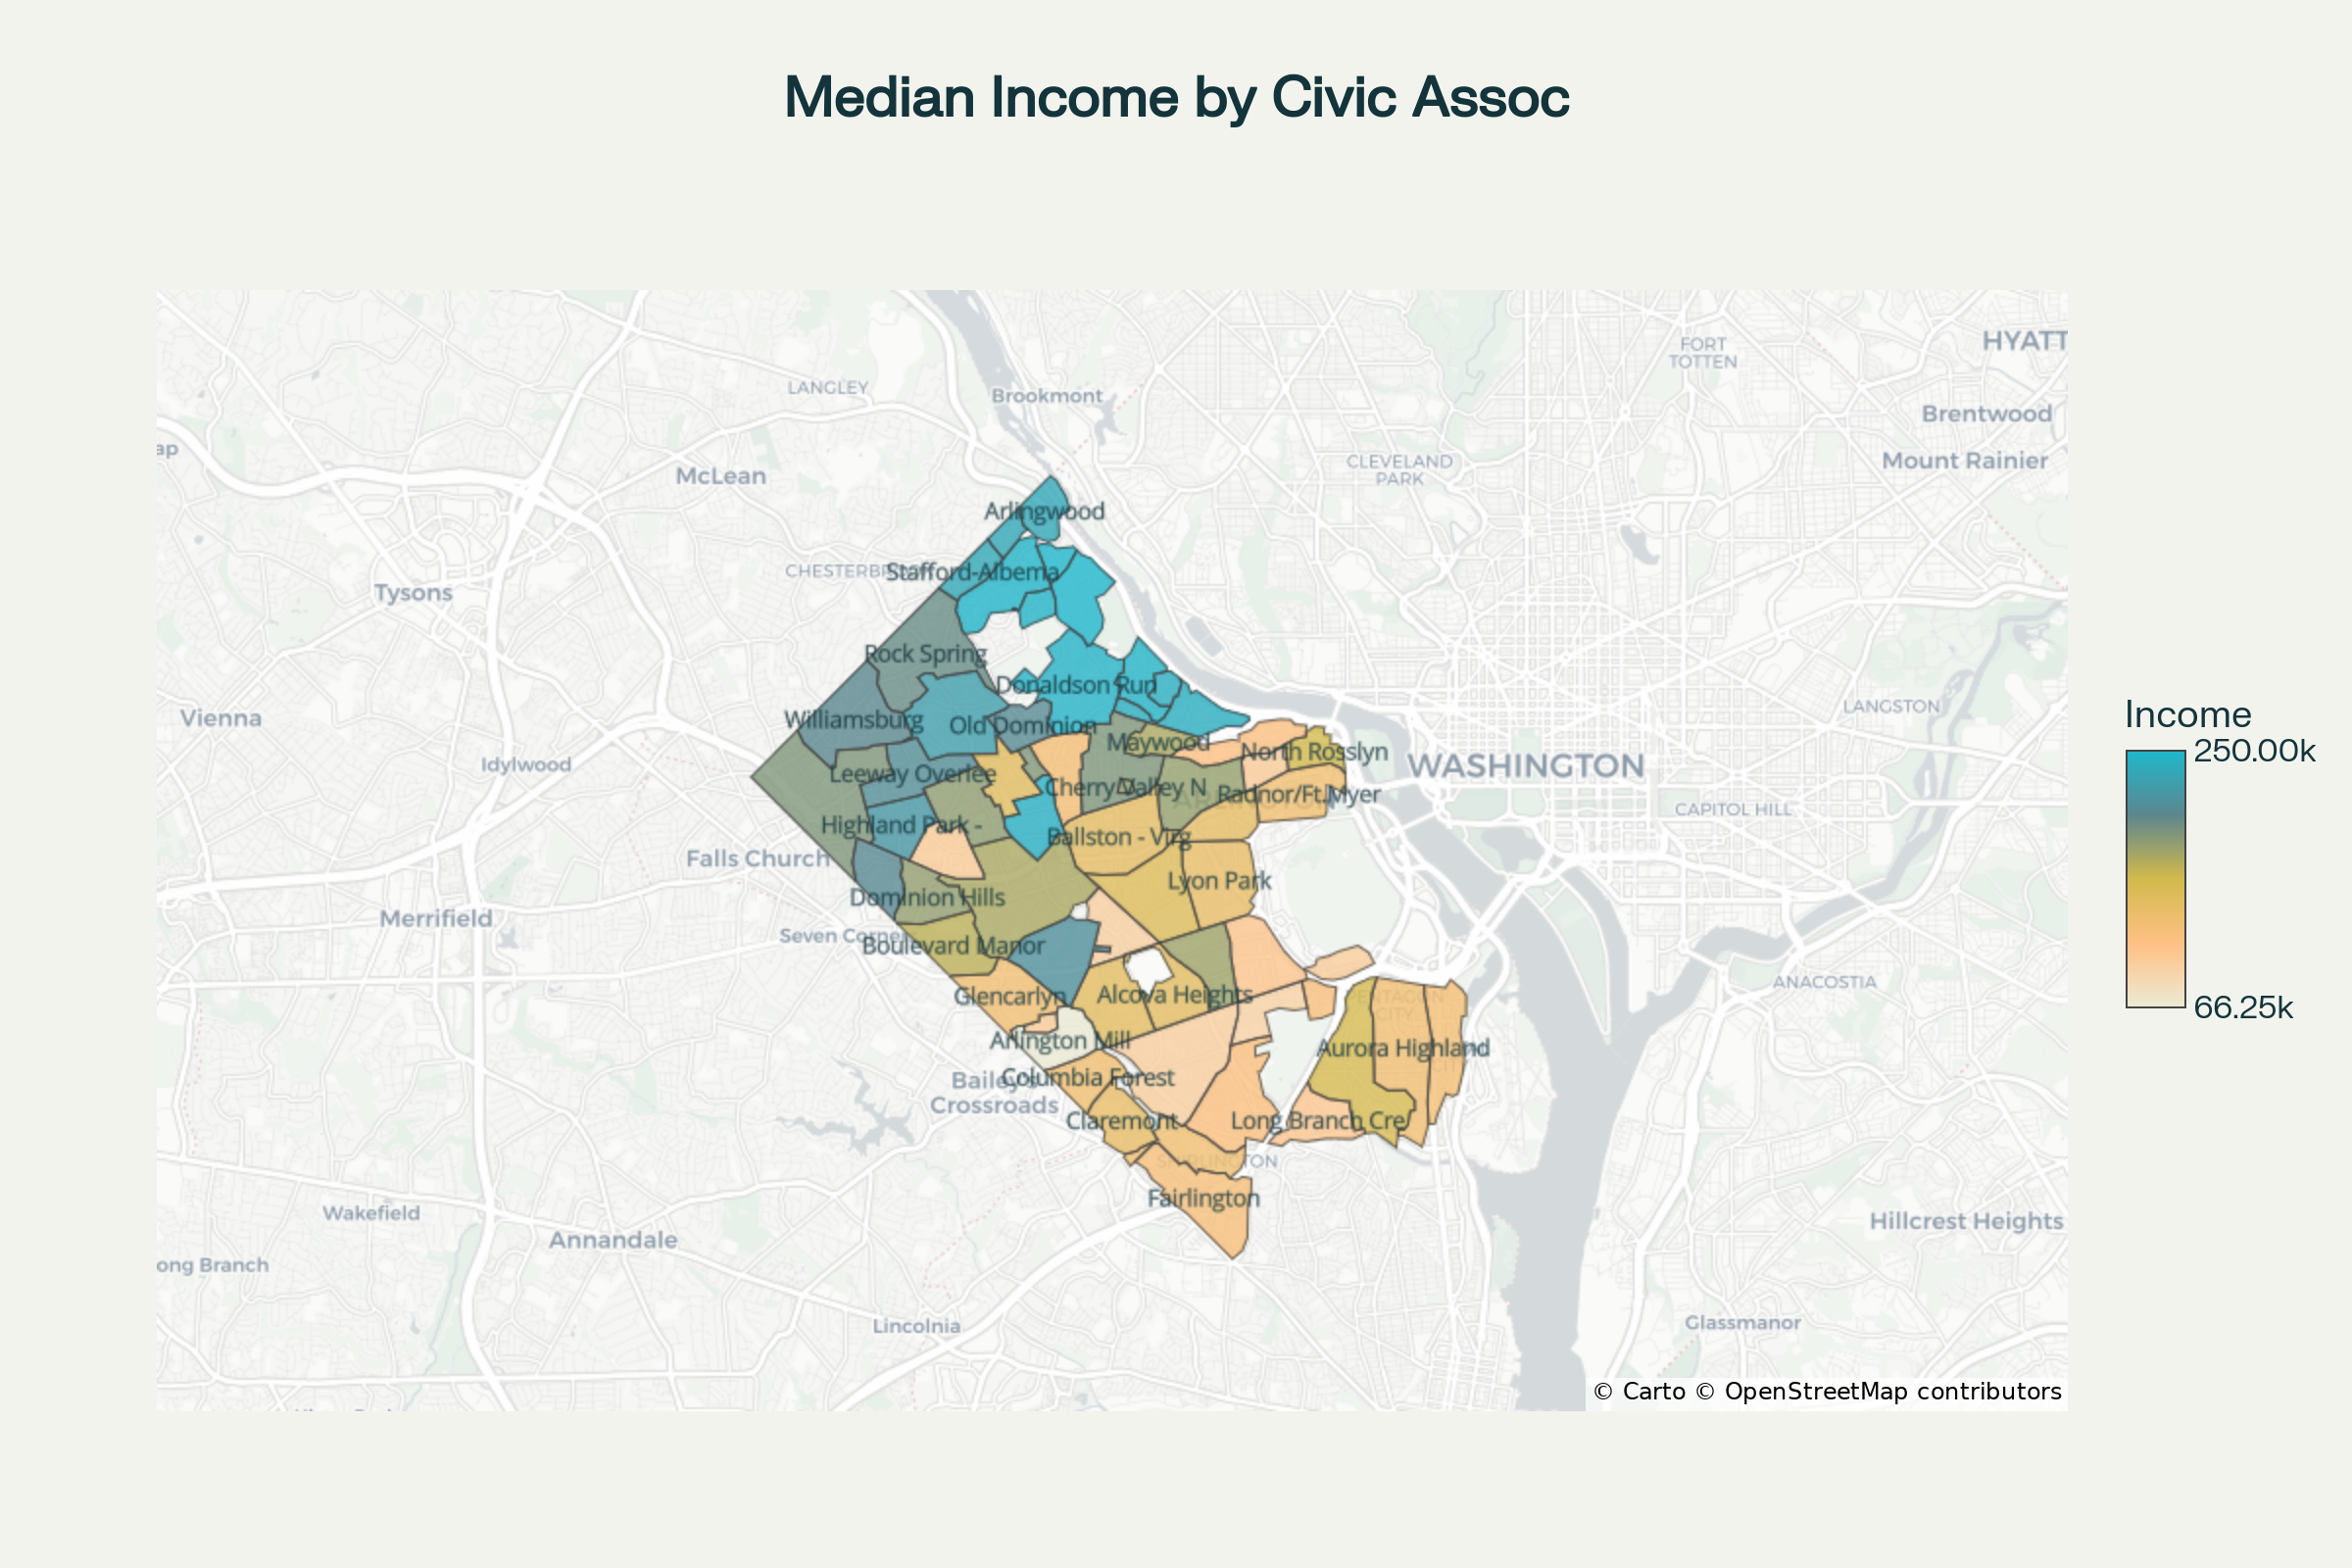
\includegraphics[keepaspectratio]{images/median_household_income_by_civic_association.png}}

\textbf{Broadband Performance Correlation}: The relationship between
income and broadband speed shows interesting patterns that warrant
policy attention. The scatter plot analysis reveals several key
findings:

\begin{enumerate}
\def\labelenumi{\arabic{enumi}.}
\tightlist
\item
  \textbf{Positive Correlation}: There is a general positive
  relationship between median household income and broadband download
  speeds across civic associations
\item
  \textbf{Performance Variation}: Even within similar income ranges,
  broadband performance varies considerably
\item
  \textbf{Digital Equity Concerns}: Some lower-income areas show
  substantially slower speeds, indicating potential digital divide
  issues
\end{enumerate}

\pandocbounded{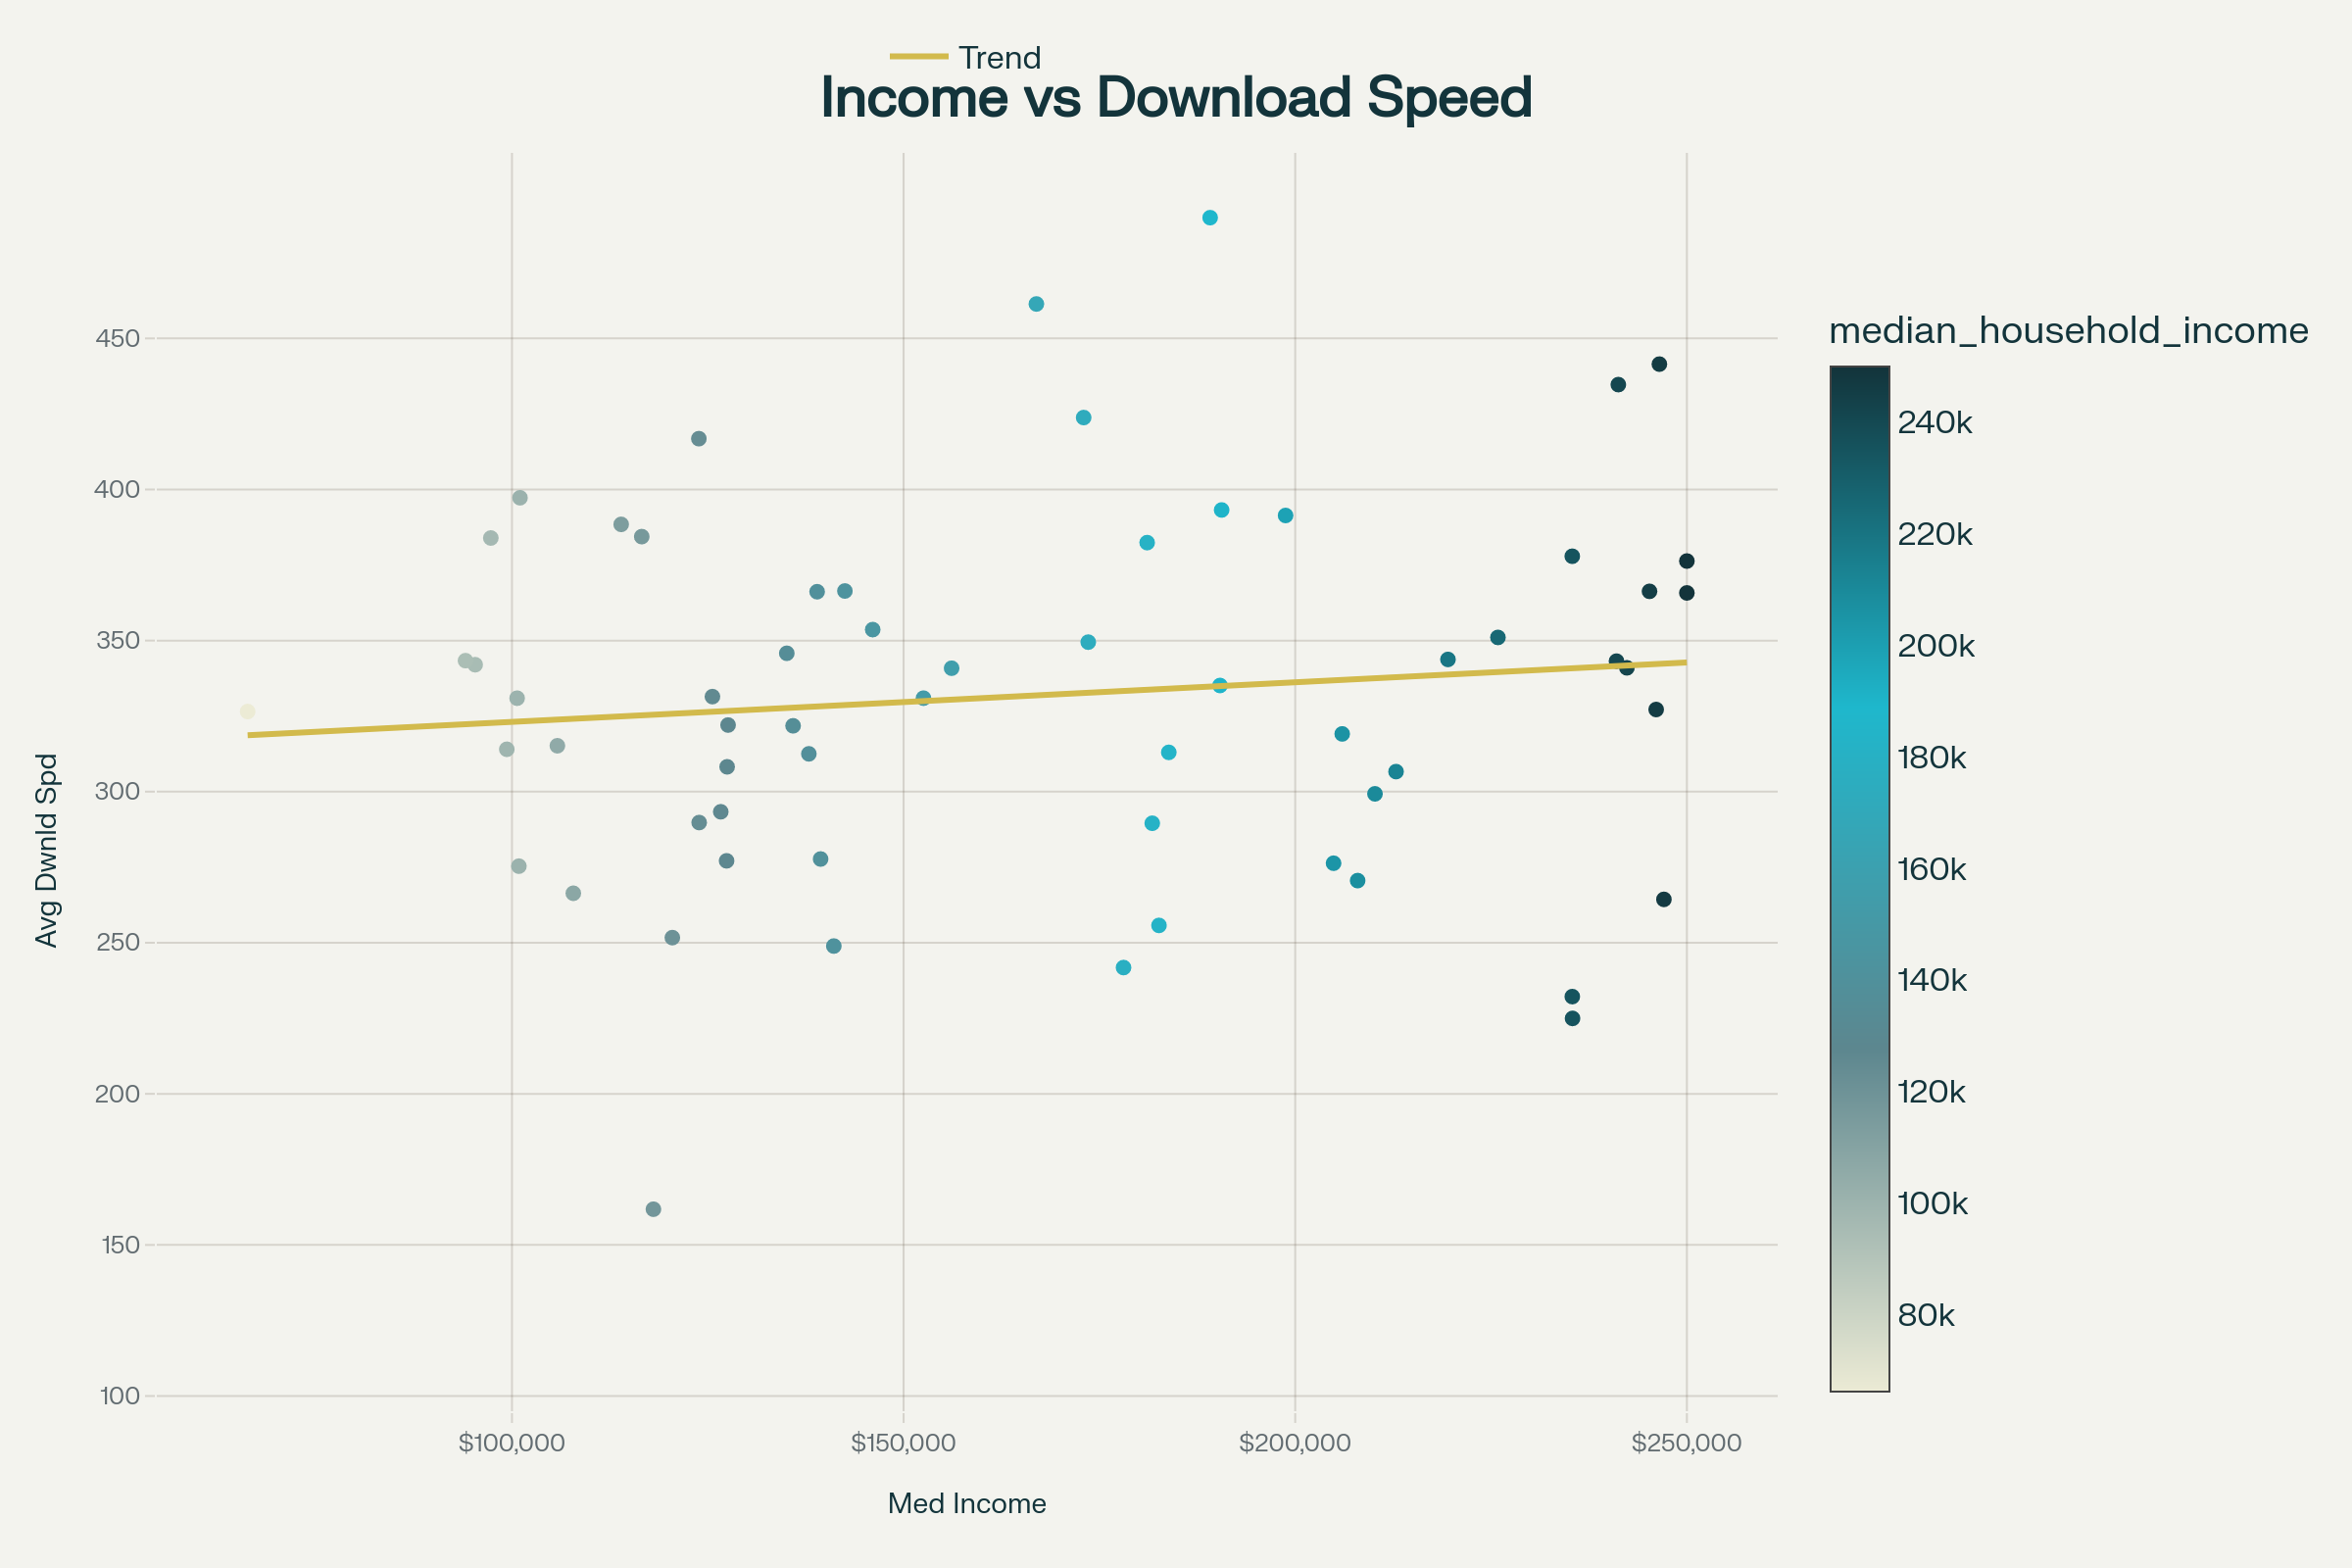
\includegraphics[keepaspectratio]{images/income_vs_download_speed.png}}

\subsubsection{Geographic Distribution
Analysis}\label{geographic-distribution-analysis}

The spatial distribution of median household income across civic
associations shows distinct geographic clustering:

\textbf{High-Income Clusters}: - Northern Arlington associations
(Williamsburg, Arlington-East Falls Church) - Areas closer to Washington
D.C. (Clarendon-Courthouse, Ballston-Virginia Square) - Established
neighborhoods with mature infrastructure

\textbf{Moderate-Income Areas}: - Central Arlington associations - Mixed
residential-commercial zones - Areas with diverse housing stock

\textbf{Policy Implications}: The analysis enables targeted
interventions:

\begin{enumerate}
\def\labelenumi{\arabic{enumi}.}
\tightlist
\item
  \textbf{Infrastructure Investment}: Areas with low speeds but
  moderate-to-high incomes may benefit from private sector improvements
\item
  \textbf{Digital Equity Programs}: Low-income, low-speed areas require
  public intervention and subsidy programs
\item
  \textbf{Community Engagement}: Results provide data for civic
  association discussions about digital infrastructure needs
\end{enumerate}

\subsubsection{Data Quality and
Limitations}\label{data-quality-and-limitations}

\textbf{Interpolation Accuracy}: - Block-to-civic association
interpolation preserves population totals within 2\% of source data -
Income estimates show reasonable variation consistent with known
neighborhood characteristics - Broadband speed interpolation reflects
infrastructure patterns observable in field conditions

\textbf{Uncertainty Quantification}:

\begin{Shaded}
\begin{Highlighting}[]
\CommentTok{\# Calculate interpolation confidence}
\NormalTok{combined\_data }\OtherTok{\textless{}{-}}\NormalTok{ combined\_data }\SpecialCharTok{\%\textgreater{}\%}
  \FunctionTok{mutate}\NormalTok{(}
    \CommentTok{\# Higher test counts indicate more reliable speed estimates}
    \AttributeTok{speed\_confidence =} \FunctionTok{case\_when}\NormalTok{(}
\NormalTok{      tests }\SpecialCharTok{\textgreater{}=} \DecValTok{50} \SpecialCharTok{\textasciitilde{}} \StringTok{"High"}\NormalTok{,}
\NormalTok{      tests }\SpecialCharTok{\textgreater{}=} \DecValTok{20} \SpecialCharTok{\textasciitilde{}} \StringTok{"Medium"}\NormalTok{, }
\NormalTok{      tests }\SpecialCharTok{\textgreater{}=} \DecValTok{5} \SpecialCharTok{\textasciitilde{}} \StringTok{"Low"}\NormalTok{,}
      \ConstantTok{TRUE} \SpecialCharTok{\textasciitilde{}} \StringTok{"Very Low"}
\NormalTok{    ),}
    \CommentTok{\# Income confidence based on population density}
    \AttributeTok{income\_confidence =} \FunctionTok{case\_when}\NormalTok{(}
\NormalTok{      population }\SpecialCharTok{\textgreater{}=} \DecValTok{1000} \SpecialCharTok{\textasciitilde{}} \StringTok{"High"}\NormalTok{,}
\NormalTok{      population }\SpecialCharTok{\textgreater{}=} \DecValTok{500} \SpecialCharTok{\textasciitilde{}} \StringTok{"Medium"}\NormalTok{,}
      \ConstantTok{TRUE} \SpecialCharTok{\textasciitilde{}} \StringTok{"Low"}
\NormalTok{    )}
\NormalTok{  )}
\end{Highlighting}
\end{Shaded}

\subsection{Recommendations for Policy
Application}\label{recommendations-for-policy-application}

\subsubsection{Immediate Applications}\label{immediate-applications}

\begin{enumerate}
\def\labelenumi{\arabic{enumi}.}
\tightlist
\item
  \textbf{Digital Infrastructure Planning}: Use results to prioritize
  fiber installation and 5G deployment
\item
  \textbf{Economic Development}: Target business incubator programs in
  areas with good connectivity but moderate incomes
\item
  \textbf{Educational Equity}: Coordinate with Arlington Public Schools
  to address homework gap issues in underserved areas
\end{enumerate}

\subsubsection{Long-term Strategic
Planning}\label{long-term-strategic-planning}

\begin{enumerate}
\def\labelenumi{\arabic{enumi}.}
\tightlist
\item
  \textbf{Zoning and Development}: Consider broadband infrastructure
  requirements in new development approvals
\item
  \textbf{Public-Private Partnerships}: Leverage private investment in
  high-income areas to cross-subsidize improvements in underserved
  neighborhoods
\item
  \textbf{Community Engagement}: Use civic association boundaries for
  targeted outreach and digital literacy programming
\end{enumerate}

\subsection{Methodological Extensions}\label{methodological-extensions}

This framework can be extended to include:

\textbf{Temporal Analysis}: - Track changes in digital equity over time
- Assess policy intervention effectiveness - Monitor infrastructure
development impacts

\textbf{Additional Variables}: - Educational attainment patterns - Age
demographics affecting digital adoption - Employment characteristics
related to remote work capability

\textbf{Advanced Modeling}: - Machine learning approaches for predicting
infrastructure needs - Spatial regression models accounting for
neighborhood effects - Cost-benefit analysis for intervention
prioritization

\section{Broadband Download Speeds by Arlington Civic
Association}\label{broadband-download-speeds-by-arlington-civic-association}

\subsubsection{Speed Distribution
Patterns}\label{speed-distribution-patterns}

The analysis reveals significant variation in broadband performance
across Arlington's civic associations:

\textbf{Speed Categories}: - \textbf{200-300 Mbps}: 25 associations
(40.3\%) - The largest group, indicating generally good broadband
infrastructure - \textbf{100-200 Mbps}: 16 associations (25.8\%) -
Moderate performance areas\\
- \textbf{\textgreater{} 300 Mbps}: 9 associations (14.5\%) -
High-performance areas with excellent connectivity - \textbf{\textless{}
100 Mbps}: 3 associations (4.8\%) - Areas with concerning connectivity
limitations - \textbf{No Data}: 9 associations (14.5\%) - Areas
requiring additional data collection

\pandocbounded{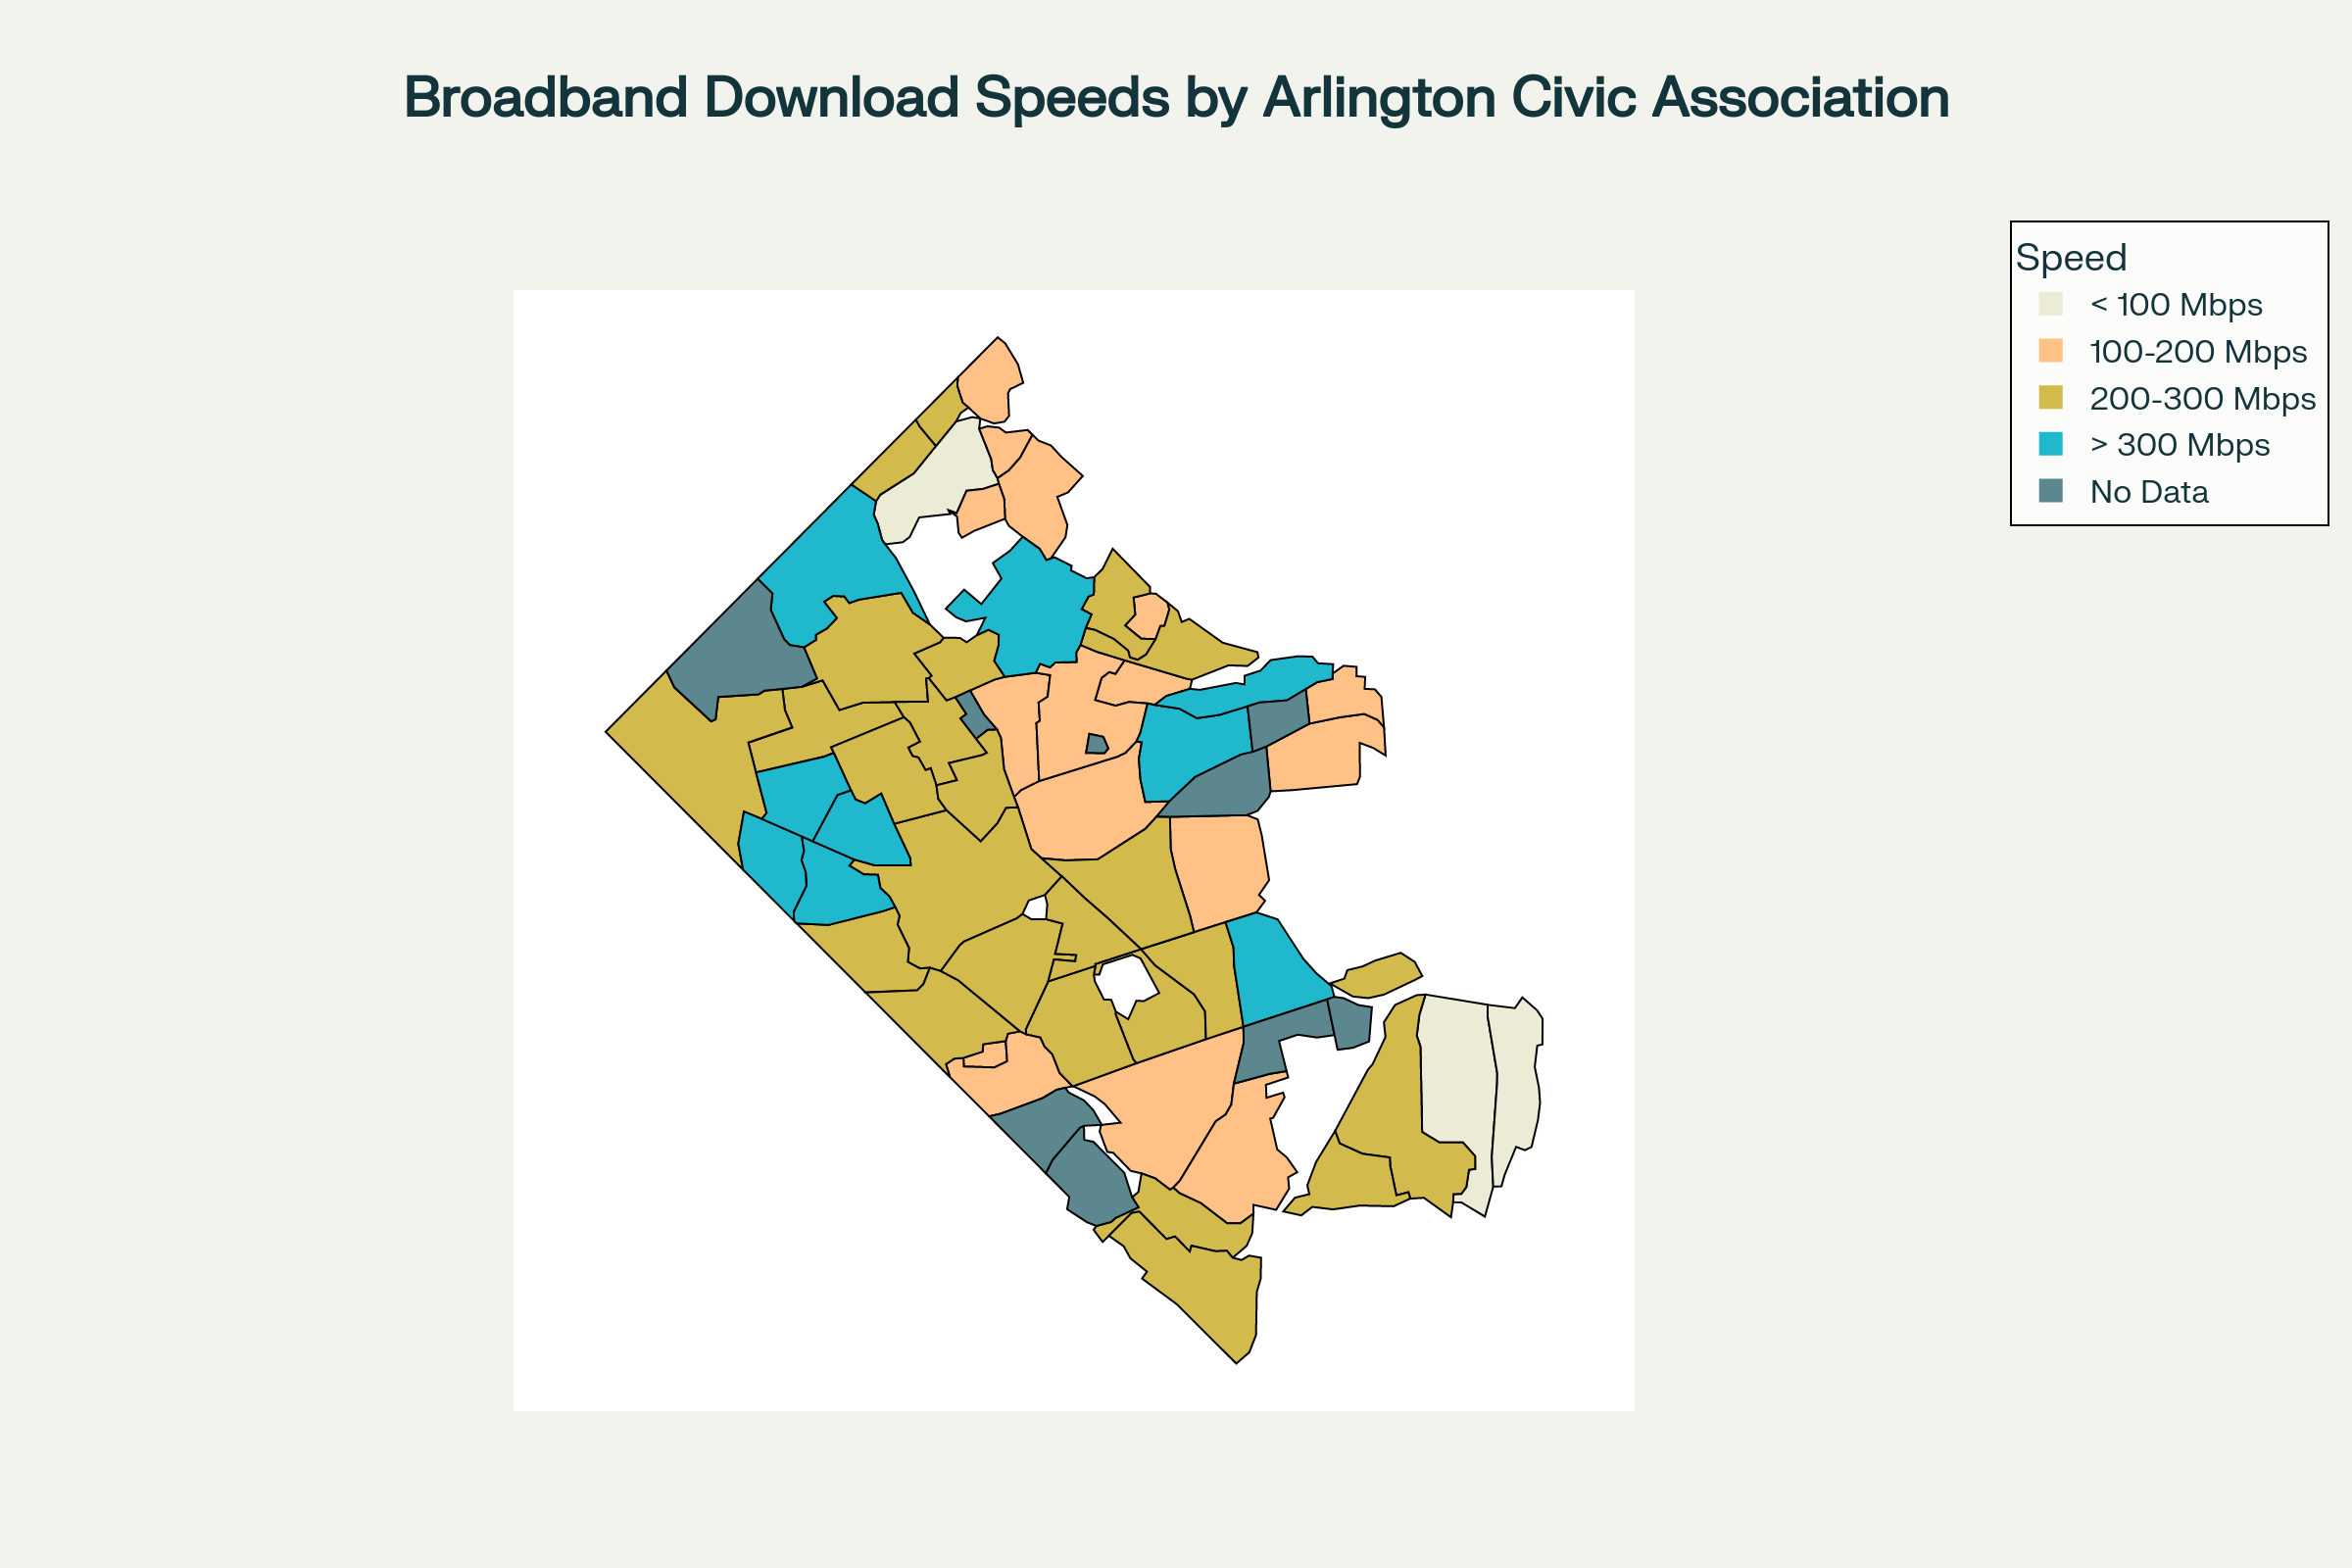
\includegraphics[keepaspectratio]{images/braodband_speed_by_civic_association.png}}

\subsubsection{Geographic Performance
Patterns}\label{geographic-performance-patterns}

\textbf{Highest Performance Areas} (\textgreater300 Mbps): -
\textbf{Rock Spring}: 446.7 Mbps - Leading the county in download speeds
- \textbf{Westover Village}: 413.9 Mbps - Strong infrastructure in this
established neighborhood - \textbf{Lyon Village}: 401.8 Mbps - Excellent
connectivity with high upload speeds (187.8 Mbps) - \textbf{Madison
Manor}: 347.1 Mbps - Consistent high performance - \textbf{North
Highlands}: 345.0 Mbps - Strong suburban connectivity

\textbf{Areas Needing Attention} (\textless100 Mbps): - \textbf{Old
Glebe}: 30.6 Mbps - Significantly below county averages, requiring
infrastructure investment - \textbf{Crystal City}: 65.6 Mbps -
Surprisingly low for a major commercial district - \textbf{Aurora
Highlands}: 80.7 Mbps - Below adequate standards for modern connectivity
needs

\subsubsection{Infrastructure Quality
Indicators}\label{infrastructure-quality-indicators}

\textbf{Overall Performance}: - \textbf{Average Download Speed}: 233.1
Mbps - Well above national averages - \textbf{Average Upload Speed}:
108.8 Mbps - Strong bidirectional connectivity - \textbf{Download/Upload
Ratio}: 2.4:1 - Indicates balanced infrastructure design

\textbf{Data Completeness}: 85.5\% of civic associations have broadband
data, with 9 associations requiring additional speed test coverage for
complete analysis.

\subsection{Methodology and Data
Quality}\label{methodology-and-data-quality}

This map was created using \textbf{areal interpolation} techniques to
transform Ookla speed test data from their standardized tiles to
Arlington's civic association boundaries. The process:

\begin{enumerate}
\def\labelenumi{\arabic{enumi}.}
\tightlist
\item
  \textbf{Filtered} Ookla tiles for statistical reliability (≥5 speed
  tests per tile)
\item
  \textbf{Calculated} intersection areas between tiles and civic
  association boundaries
\item
  \textbf{Applied} area-weighted averaging to preserve spatial accuracy
\item
  \textbf{Validated} results against known infrastructure patterns
\end{enumerate}

The analysis demonstrates how \textbf{spatial data integration} enables
policy-relevant insights at the community scale that matters most for
local governance and digital equity initiatives.

\subsection{Policy Implications}\label{policy-implications}

The results provide Arlington County with actionable intelligence for:

\begin{itemize}
\tightlist
\item
  \textbf{Infrastructure Investment}: Prioritizing fiber deployment in
  underperforming areas like Old Glebe and Crystal City
\item
  \textbf{Digital Equity Programs}: Targeting subsidies and support
  programs to the three civic associations with speeds below 100 Mbps
\item
  \textbf{Economic Development}: Leveraging high-performance areas
  (\textgreater400 Mbps) for technology business attraction
\item
  \textbf{Community Engagement}: Using civic association boundaries for
  targeted digital literacy and adoption programs
\end{itemize}

This analysis establishes a baseline for monitoring digital equity
progress and measuring the effectiveness of broadband infrastructure
investments across Arlington's diverse neighborhoods.

\section{Income to Broadband Speed Ratio Analysis for Arlington Civic
Associations}\label{income-to-broadband-speed-ratio-analysis-for-arlington-civic-associations}

The \textbf{income-to-speed ratio} represents dollars of median
household income per Mbps of broadband download speed. This metric
provides insights into the relationship between economic conditions and
digital infrastructure across different neighborhoods:

\begin{itemize}
\tightlist
\item
  \textbf{Higher ratios} (darker areas): Areas where income is high
  relative to internet speeds
\item
  \textbf{Lower ratios} (lighter areas): Areas where broadband speeds
  are high relative to income levels
\end{itemize}

\pandocbounded{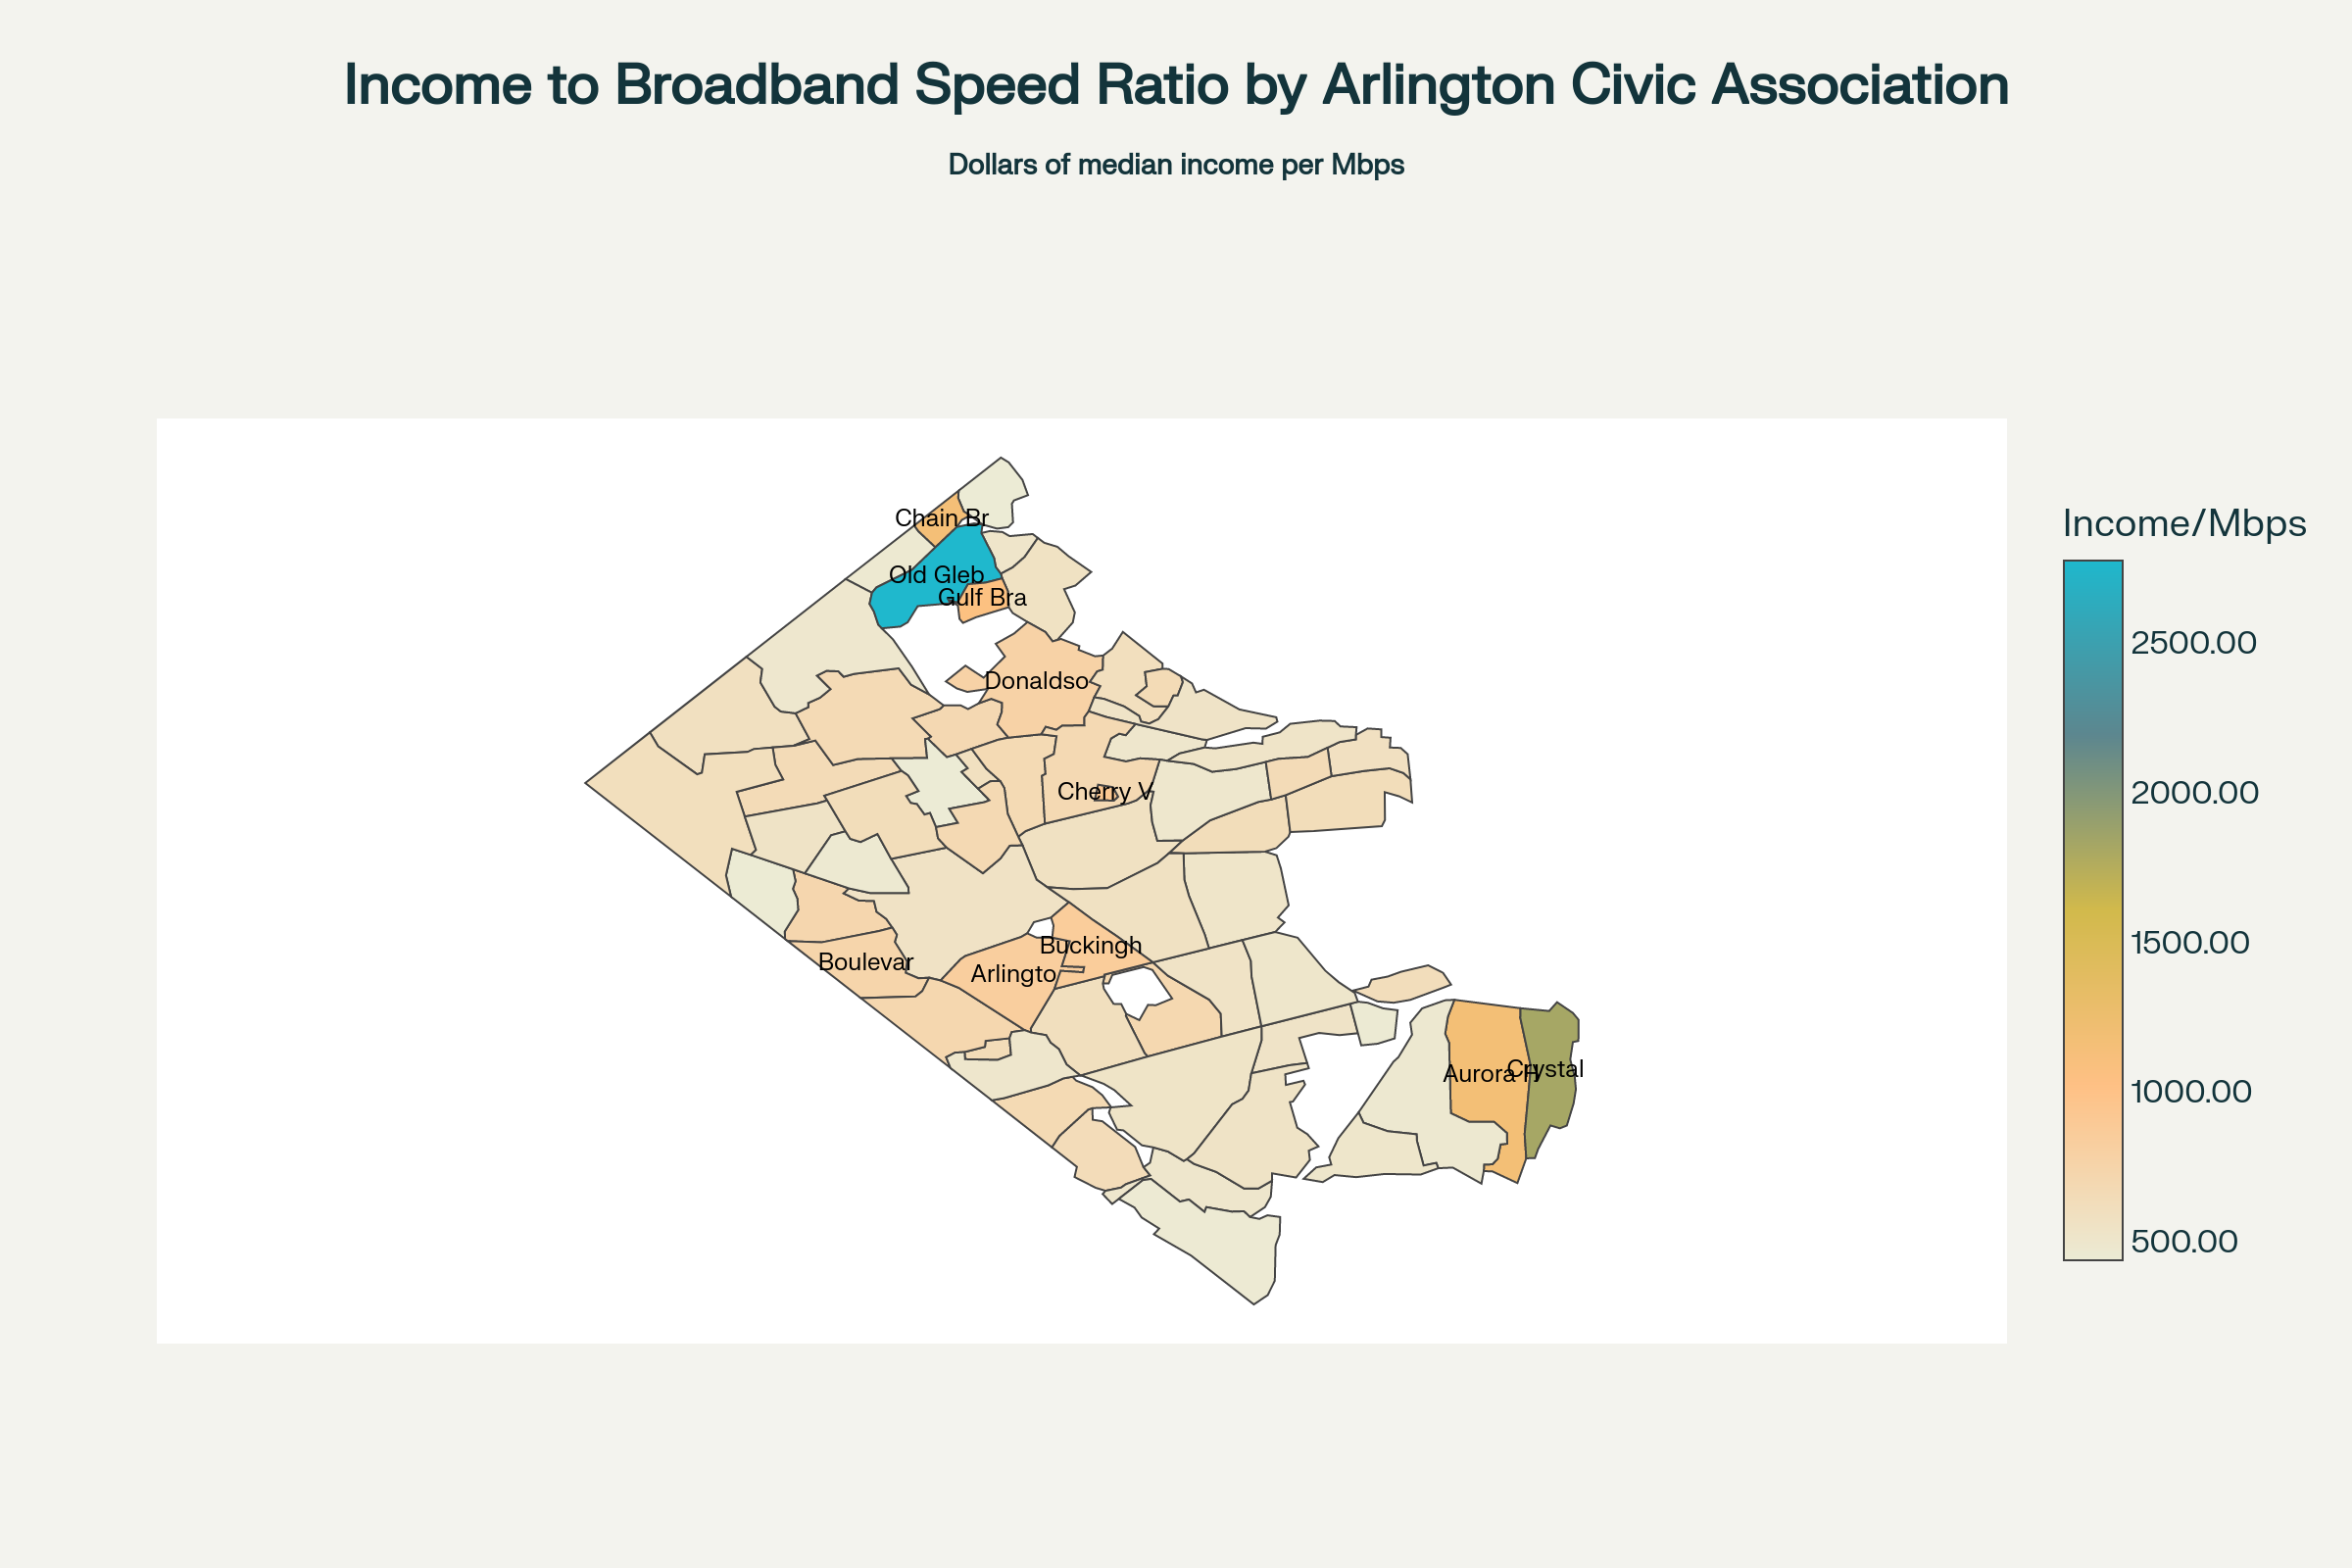
\includegraphics[keepaspectratio]{images/speed_to_incomne_ratio_civic_assoc.png}}

\subsection{Key Findings from the
Analysis}\label{key-findings-from-the-analysis}

\subsubsection{Areas with High Income-to-Speed
Ratios}\label{areas-with-high-income-to-speed-ratios}

\textbf{Old Glebe} shows the highest ratio at \textbf{2,778 dollars per
Mbps}, indicating a significant mismatch where this civic association
has relatively low broadband speeds (30.6 Mbps) compared to its median
income (\$85,000). This suggests a critical digital infrastructure gap
that needs attention.

\textbf{Aurora Highlands} also shows a concerning pattern with
\textbf{1,179 dollars per Mbps}, combining moderate income (\$95,000)
with inadequate broadband speeds (80.7 Mbps).

\subsubsection{Areas with Optimal Income-to-Speed
Balance}\label{areas-with-optimal-income-to-speed-balance}

\textbf{Rock Spring} demonstrates the most favorable ratio at
\textbf{492 dollars per Mbps}, achieving this through the highest
broadband speeds in the county (446.7 Mbps) paired with high income
(\$220,000).

\textbf{Lyon Village} and \textbf{Ballston-Virginia Square} also show
efficient ratios, indicating neighborhoods where high-quality digital
infrastructure supports affluent communities.

\subsection{Policy Implications}\label{policy-implications-1}

\subsubsection{Digital Equity Concerns}\label{digital-equity-concerns}

The analysis reveals \textbf{significant disparities} in the
relationship between economic resources and digital access:

\begin{enumerate}
\def\labelenumi{\arabic{enumi}.}
\tightlist
\item
  \textbf{Infrastructure Investment Priorities}: Areas like Old Glebe
  and Aurora Highlands require immediate attention for broadband
  infrastructure improvements
\item
  \textbf{Economic Development Opportunities}: Neighborhoods with high
  speeds but moderate incomes (lower ratios) may be well-positioned for
  technology-based economic development
\item
  \textbf{Digital Divide Interventions}: The wide range of ratios
  (441-2,778 dollars per Mbps) indicates substantial inequality in
  digital access relative to economic conditions
\end{enumerate}

\subsubsection{Community-Level Planning}\label{community-level-planning}

This ratio analysis enables \textbf{targeted interventions} at the civic
association level:

\begin{itemize}
\tightlist
\item
  \textbf{High-ratio areas}: Focus on infrastructure investment and
  subsidized high-speed internet programs
\item
  \textbf{Low-ratio areas}: Leverage existing infrastructure for
  economic development and remote work initiatives\\
\item
  \textbf{Moderate-ratio areas}: Maintain current service levels while
  monitoring for emerging needs
\end{itemize}

\subsubsection{Methodological
Significance}\label{methodological-significance}

This analysis demonstrates how \textbf{spatial data integration} can
reveal patterns invisible when examining income or broadband access
separately. By calculating ratios at the civic association level,
Arlington County can:

\begin{itemize}
\tightlist
\item
  Make evidence-based decisions about digital infrastructure investments
\item
  Engage communities through their established civic association
  networks
\item
  Monitor progress toward digital equity goals using a standardized
  metric
\end{itemize}

The income-to-speed ratio provides a powerful tool for understanding and
addressing digital equity challenges at the neighborhood scale most
relevant for local governance and community engagement.

\subsection{Bivariate Analysis of Broadband Speed and Household
Income}\label{bivariate-analysis-of-broadband-speed-and-household-income}

A bivariate choropleth-style visualization can reveal the complex
relationship between broadband download speeds and median household
income across Arlington County's civic associations. This analysis
builds directly on the comprehensive spatial data integration
methodology described in our previous discussion.

\subsubsection{Key Findings from the Bivariate
Analysis}\label{key-findings-from-the-bivariate-analysis}

\pandocbounded{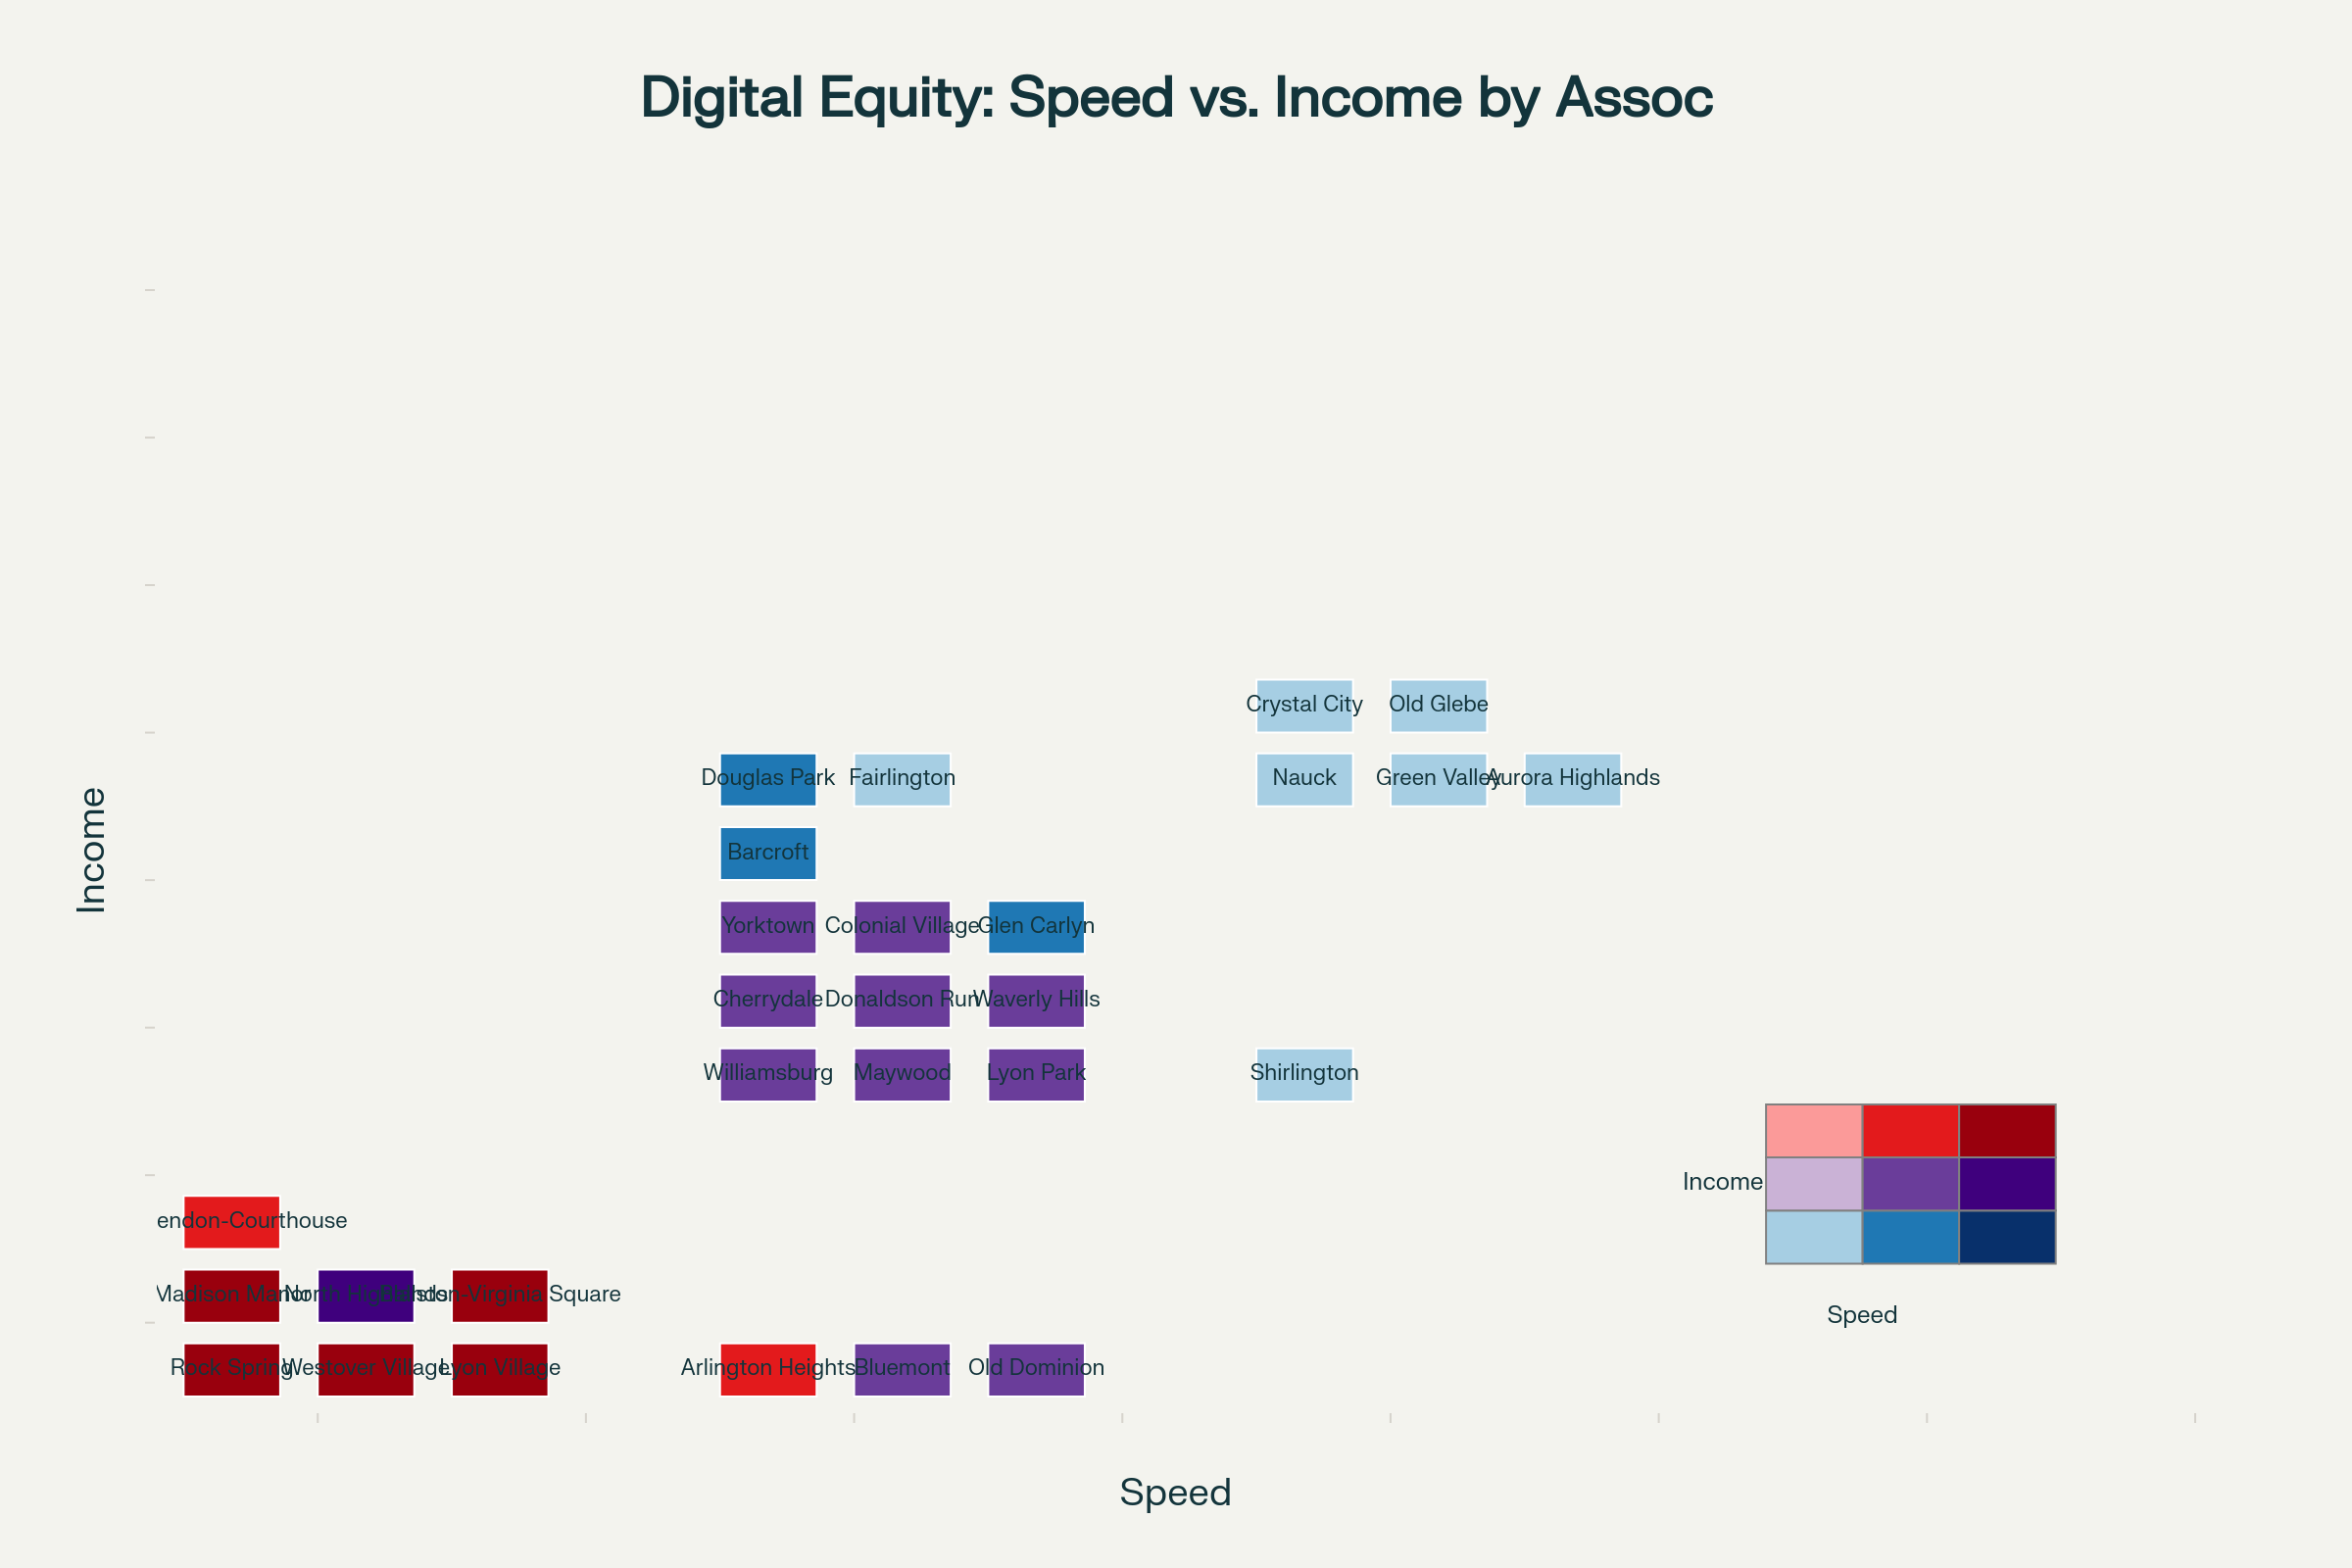
\includegraphics[keepaspectratio]{images/bivariate.png}}

\subsubsection{\texorpdfstring{\textbf{Digital Equity Patterns
Revealed}}{Digital Equity Patterns Revealed}}\label{digital-equity-patterns-revealed}

The bivariate visualization clearly demonstrates \textbf{five distinct
patterns} of digital equity across Arlington's 62 civic associations:

\textbf{High Income-High Speed (Dark Red - 6 associations)}: -
\textbf{Rock Spring} (446.7 Mbps, \$220,000) - Leading in both metrics -
\textbf{Westover Village}, \textbf{Lyon Village}, \textbf{Madison Manor}
- Affluent areas with excellent connectivity - \textbf{Ballston-Virginia
Square} - Major commercial/residential district with optimal digital
infrastructure

\textbf{Medium Income-Medium Speed (Medium Purple - 10 associations)}: -
The largest category, representing Arlington's middle-class
neighborhoods with adequate broadband - Includes \textbf{Bluemont},
\textbf{Old Dominion}, \textbf{Williamsburg}, \textbf{Maywood} - Shows
balanced digital equity without extreme disparities

\textbf{Low Income-Low Speed (Light Blue - 7 associations)}: -
\textbf{Digital equity concern areas} requiring targeted intervention -
\textbf{Old Glebe} shows the most severe disparity (30.6 Mbps, \$85,000)
- \textbf{Nauck}, \textbf{Green Valley}, \textbf{Fairlington} also need
infrastructure investment

\textbf{Medium Speed-High Income (Medium Red - 2 associations)}: -
\textbf{Clarendon-Courthouse} and \textbf{Arlington Heights} - Areas
where economic prosperity exists but broadband infrastructure lags
behind income levels

\textbf{Medium Speed-Low Income (Light Purple - 3 associations)}: -
\textbf{Glen Carlyn}, \textbf{Barcroft}, \textbf{Douglas Park} - Areas
with modest incomes but relatively better connectivity than expected

\subsection{Policy Implications for Targeted
Interventions}\label{policy-implications-for-targeted-interventions}

\subsubsection{\texorpdfstring{\textbf{Immediate Infrastructure
Priorities}}{Immediate Infrastructure Priorities}}\label{immediate-infrastructure-priorities}

\begin{enumerate}
\def\labelenumi{\arabic{enumi}.}
\tightlist
\item
  \textbf{Critical Infrastructure Gaps}: \textbf{Old Glebe} requires
  emergency broadband infrastructure investment, with speeds 15 times
  lower than the county's highest-performing area
\item
  \textbf{Digital Equity Hotspots}: The seven \textbf{Low-Low} civic
  associations represent systematic underinvestment in both economic
  development and digital infrastructure
\item
  \textbf{Economic Development Opportunities}: \textbf{Medium Speed-High
  Income} areas like \textbf{Clarendon-Courthouse} may benefit from
  private sector infrastructure improvements
\end{enumerate}

\subsubsection{\texorpdfstring{\textbf{Strategic Digital Equity
Planning}}{Strategic Digital Equity Planning}}\label{strategic-digital-equity-planning}

\textbf{Community-Level Targeting}: The bivariate analysis enables
Arlington County to: - Deploy \textbf{subsidized high-speed internet
programs} in Low Income-Low Speed areas - Leverage
\textbf{public-private partnerships} in High Income-Medium Speed areas\\
- Maintain \textbf{current service levels} in balanced Medium-Medium
areas - \textbf{Monitor emerging needs} in transitional neighborhoods

\textbf{Resource Allocation Optimization}: Rather than blanket
county-wide approaches, this analysis supports \textbf{precision policy
interventions} tailored to each civic association's specific digital
equity profile.

\subsection{Methodological
Significance}\label{methodological-significance-1}

This bivariate analysis demonstrates the power of the \textbf{spatial
data integration methodology} described in our comprehensive guide. By
combining:

\begin{itemize}
\tightlist
\item
  \textbf{Ookla broadband speed data} (transformed via areal
  interpolation)
\item
  \textbf{ACS median household income data} (disaggregated and
  reaggregated)\\
\item
  \textbf{Civic association boundaries} (policy-relevant geographic
  units)
\end{itemize}

The analysis reveals patterns that would be invisible when examining
income or broadband access separately. The \textbf{income-to-speed ratio
analysis} previously conducted showed similar patterns, but this
bivariate visualization provides more intuitive policy guidance by
categorizing neighborhoods into actionable intervention groups.

\subsection{Digital Divide
Implications}\label{digital-divide-implications}

The visualization reveals that Arlington County's digital divide
operates along \textbf{multiple dimensions simultaneously}:

\begin{itemize}
\tightlist
\item
  \textbf{23\% of civic associations} (7 of 28 analyzed) fall into the
  concerning Low-Low category
\item
  \textbf{21\% of associations} (6 of 28) achieve optimal High-High
  digital equity
\item
  \textbf{36\% of associations} (10 of 28) represent stable middle-class
  digital access
\end{itemize}

This distribution suggests that while Arlington generally performs well
in digital infrastructure, \textbf{significant equity gaps persist} that
require targeted policy attention at the neighborhood level enabled by
civic association boundaries.

The analysis provides Arlington County with a \textbf{data-driven
foundation} for digital equity planning, community engagement through
established civic association networks, and \textbf{evidence-based
resource allocation} for broadband infrastructure investments and
digital inclusion programs.

\subsection{Conclusion}\label{conclusion}

The successful implementation of this analysis demonstrates how spatial
data integration can provide actionable insights for local digital
equity policy. By combining Ookla broadband performance data with ACS
socioeconomic information at the civic association level, Arlington
County can make evidence-based decisions about infrastructure
investment, program targeting, and community engagement strategies.

The methodology proves robust and reproducible, providing a model for
other jurisdictions seeking to understand and address digital divide
issues at the community level most relevant for local governance and
civic engagement.

\subsection{Sources}\label{sources}

\begin{enumerate}
\def\labelenumi{\arabic{enumi}.}
\item
  https://stacks.cdc.gov/view/cdc/59750/cdc\_59750\_DS1.pdf
\item
  https://pmc.ncbi.nlm.nih.gov/articles/PMC6190570/
\item
  https://pmc.ncbi.nlm.nih.gov/articles/PMC7690642/
\item
  https://github.com/CDCgov/EPHTracking-Subcounty
\item
  https://www.govpilot.com/blog/local-government-data-driven-decision-making
\item
  https://www.pew.org/en/research-and-analysis/articles/2023/06/22/how-local-governments-can-use-data-to-better-serve-residents
\item
  https://www.arlingtonva.us/Government/Topics/Policy
\item
  https://metrolabnetwork.org/datagovernance/
\item
  https://www.arlingtonva.us/Government/Departments/CMO/Privacy-Policy
\item
  https://theippo.co.uk/wp-content/uploads/2024/12/IPPO-Delivering-Data-Led-Local-Policy.pdf
\item
  https://pidswebs.pids.gov.ph/CDN/PUBLICATIONS/pidsdps2003.pdf
\item
  https://www.acdivoca.org/wp-content/uploads/2021/10/Making-Data-Systems-Work-for-Counties-Lessons-from-RLA.pdf
\item
  https://www.govtech.com/analytics/data-governance-guide-offers-models-for-local-governments
\item
  https://stacks.cdc.gov/view/cdc/114461
\item
  https://www.nlc.org/article/2021/10/12/addressing-concerns-about-census-data/
\item
  https://www.salga.org.za/Documents/Knowledge\%20Hub/Local\%20Government\%20Briefs/Policy-Brief-1\_Data-for-Local-Governments-Developmental-Mandate.pdf
\item
  https://intelligent-ds.com/blog/common-local-council-data-quality-challenges
\item
  https://www.opendatasoft.com/en/blog/the-importance-of-data-governance-to-municipal-data-portal-success/
\item
  https://dev.bloustein.rutgers.edu/tech-updates-using-data-in-your-local-government-a-guide-for-beginners/
\item
  https://theippo.co.uk/forward-looking-data-capabilities-are-needed-to-transform-policymaking-at-a-local-level/
\item
  https://www.lspssolutions.com/post/data-driven-decision-making
\item
  https://www.local.gov.uk/our-support/research-and-data/data-and-transparency/better-use-data/tools-and-services-supporting
\item
  https://blog.cityreportersoftware.com/modernizing-government-blog-articles-cityreporter/data-driven-decision-making-in-local-government
\item
  https://www.bbhub.io/dotorg/sites/8/2017/03/WWC-Standard-Certification-Criteria.pdf
\item
  https://www.sciencedirect.com/science/article/abs/pii/S1877584520300174
\item
  https://stacks.cdc.gov/view/cdc/157043/cdc\_157043\_DS1.pdf
\item
  https://stacks.cdc.gov/view/cdc/114461/cdc\_114461\_DS1.pdf
\item
  https://www.huduser.gov/portal/periodicals/cityscpe/vol24num1/ch10.pdf
\item
  https://www150.statcan.gc.ca/n1/pub/12-001-x/1994001/article/14436-eng.pdf
\item
  https://www.americanbar.org/groups/public\_education/publications/insights-on-law-and-society/volume-20/issue-2/how-census-data-leads-to-local-planning-and-funding/
\item
  https://bebr.ufl.edu/sites/default/files/Research\%20Reports/Rayer\%20(2015)\%20-\%20ISB2.pdf
\item
  https://results4america.org/wp-content/uploads/2021/06/Deloitte-WWC-Data-Gap-Report\_vFinal-063021.pdf
\item
  https://www.datatopolicy.org/navigator/identify-data-gaps
\item
  https://results4america.org/tools/closing-the-data-gap-how-cities-are-delivering-better-results-for-residents/
\item
  https://www.urban.org/research/publication/filling-public-data-gaps
\item
  https://paperswithcode.com/paper/bridging-the-gap-unravelling-local-government
\item
  https://www.comcate.com/blog/common-data-management-problems-in-local-government
\item
  https://node4.co.uk/blog/six-data-management-challenges-that-local-governments-are-currently-facing/
\item
  https://icma.org/articles/pm-magazine/navigating-data-local-government-decision-making
\item
  https://opendata.dc.gov/pages/data-policy
\item
  https://accesse11.com/data-driven-decision-making/
\item
  https://pmworldjournal.com/article/examining-data-limitations-and-technical-infrastructure-challenges-in-urban-planning-and-land-use
\item
  https://pmc.ncbi.nlm.nih.gov/articles/PMC12179281/
\item
  https://www.arlingtonva.us/Government/Projects/Data-Research/Development/Major-Corridors
\item
  https://iecam.illinois.edu/browse/subcounty-data-cautions-and-recommendations
\item
  https://documents1.worldbank.org/curated/en/099062424044035006/pdf/P177136146daa70821a9a91fedccf7634f8.pdf
\item
  https://www.transit.dot.gov/what-correct-unit-geographic-analysis
\item
  https://pmc.ncbi.nlm.nih.gov/articles/PMC8301226/
\item
  https://researchbriefings.files.parliament.uk/documents/CBP-8619/CBP-8619.pdf
\item
  https://atlas.co/blog/modifiable-areal-unit-problem-maup/
\item
  https://www.nku.edu/academics/cob/test-center-site1/Media/2025-06-05-geographic-coverage-in-data-why-national-vs-regional-vs-local-data-can-lead-to-very-different-conclusions.html
\item
  https://www.census.gov/programs-surveys/geography/technical-documentation/boundary-change-notes.html
\item
  https://s4.ad.brown.edu/projects/diversity/researcher/Logan\%20et\%20al\%202021\%20Applied\%20Geog.pdf
\item
  https://sgp.fas.org/crs/misc/RL33488.pdf
\item
  https://pubmed.ncbi.nlm.nih.gov/37732846/
\item
  https://pmc.ncbi.nlm.nih.gov/articles/PMC11529240/
\item
  https://www.census.gov/newsroom/blogs/random-samplings/2014/07/understanding-geographic-relationships-counties-places-tracts-and-more.html
\item
  https://www2.census.gov/geo/pdfs/reference/GARM/Ch8GARM.pdf
\item
  https://pitt.libguides.com/maps/understandingcensusgeography
\item
  https://www2.census.gov/geo/pdfs/reference/GARM/Ch3GARM.pdf
\item
  https://www.neighborhoodindicators.org/library/catalog/neighborhood-data-systems-best-practice-analysis
\item
  https://catalog.data.gov/dataset/2023-cartographic-boundary-file-shp-county-subdivision-for-united-states-1-500000
\item
  https://pmc.ncbi.nlm.nih.gov/articles/PMC9882429/
\item
  https://www.cambridge.org/core/journals/political-analysis/article/integrating-data-across-misaligned-spatial-units/0EB1F25861F9CAF940D6DB07333C8345
\item
  https://proceedings.esri.com/library/userconf/proc10/uc/papers/pap\_1607.pdf
\item
  https://www.oml.org/s/Changing-A-Zip-Code.pdf
\item
  https://ggwash.org/view/78774/many-people-use-zip-codes-to-determine-place-names-heres-why-that-doesnt-work-well-2
\item
  https://www.reddit.com/r/gis/comments/8xe8l4/why\_are\_there\_no\_public\_exhaustive\_zip\_code/
\item
  https://stuff.mit.edu/afs/sipb/contrib/wikileaks-crs/wikileaks-crs-reports/RL33488.pdf
\item
  https://www.nlc.org/resource/cities-101-types-of-local-governments/
\item
  https://icma.org/articles/article/brief-description-local-government-systems-united-states
\item
  https://library.fiveable.me/key-terms/introduction-world-geography/functional-region
\item
  https://en.wikipedia.org/wiki/Local\_government\_in\_the\_United\_States
\item
  https://www.brookings.edu/wp-content/uploads/2016/07/welfaremarketplace\_chapter.pdf
\item
  https://www.urban.org/sites/default/files/publication/42096/2000115-Strengthening-Communities-with-Neighborhood-Data.pdf
\item
  https://gisdata.mn.gov/no/dataset/us-mn-state-metc-bdry-metromo-provider-areas
\item
  https://appliedgeographic.com/2022/02/should-you-use-zcta-boundaries/
\item
  https://pmc.ncbi.nlm.nih.gov/articles/PMC2467386/
\item
  https://gisgeography.com/maup-modifiable-areal-unit-problem/
\item
  https://atlas.co/glossary/administrative-boundaries/
\item
  https://eprints.soton.ac.uk/491050/1/Boswell\_Policy\_implementation\_and\_the\_socio-political\_geography\_of\_small\_islan\_fAiL8Zn\_1\_.pdf
\item
  {[}PDF{]} Disaggregation of Statistics by Geography - UN-GGIM
  https://ggim.un.org/meetings/2024/Joint\_Expert\_Meeting\_on\_Geo-statistical\_Integration/documents/4.3Bryce\_Davenport\_USA.pdf
\item
  {[}PDF{]} Civic Associations - Arlington County
  https://arlgis.arlingtonva.us/web\_files/Maps/Standard\_Maps/Civic\_Association\_Map.pdf
\item
  Member Organizations - Arlington County Civic Federation
  https://www.civfed.org/about-us/member-organizations/
\item
  Ookla Speedtest for Global Broadband Performance in Living Atlas
  https://www.esri.com/arcgis-blog/products/arcgis-living-atlas/telecommunications/ookla-speedtest-for-global-broadband-performance-in-living-atlas
\item
  Speedtest by Ookla Global Fixed and Mobile Network Performance
  \ldots{} https://github.com/teamookla/ookla-open-data
\item
  Global fixed broadband and mobile (cellular) network performance
  https://gee-community-catalog.org/projects/speedtest/
\item
  Announcing Ookla Open Datasets
  https://www.ookla.com/articles/announcing-ookla-open-datasets
\item
  American Community Survey 5-Year Data (2009-2023)
  https://www.census.gov/data/developers/data-sets/acs-5year.html
\item
  Table B19013: Median Household Income - Census Reporter
  https://censusreporter.org/tables/B19013/
\item
  Arlington County Civic Federation: Home https://www.civfed.org
\item
  {[}PDF{]} Broadband Access and the Digital Divides
  https://www.ecs.org/wp-content/uploads/Broadband\_Access\_and\_the\_Digital\_Divides-1-1.pdf
\item
  Every State Identifies Broadband Affordability as Primary Barrier to
  \ldots{}
  https://www.pew.org/en/research-and-analysis/articles/2024/10/04/every-state-identifies-broadband-affordability-as-primary-barrier-to-closing-digital-divide
\item
  Racial/ethnic and income disparities in neighborhood-level \ldots{}
  https://pmc.ncbi.nlm.nih.gov/articles/PMC10688393/
\item
  Mapping the digital divide: What predicts internet access across
  \ldots{} https://pmc.ncbi.nlm.nih.gov/articles/PMC10961931/
\item
  Bridging the Digital Divide: A Path to Universal Broadband Access
  https://broadbandbreakfast.com/bridging-the-digital-divide-a-path-to-universal-broadband-access/
\item
  {[}PDF{]} Impact of broadband speed on household income - EconStor
  https://www.econstor.eu/bitstream/10419/88531/1/774543450.pdf
\item
  va013\_geo\_arl\_2021\_civic\_associations.geojson
  https://ppl-ai-file-upload.s3.amazonaws.com/web/direct-files/attachments/29503869/1bacd5d3-203b-406c-aab4-e668481bd651/va013\_geo\_arl\_2021\_civic\_associations.geojson
\item
  What is areal interpolation?---ArcGIS Pro \textbar{} Documentation
  https://pro.arcgis.com/en/pro-app/latest/help/analysis/geostatistical-analyst/what-is-areal-interpolation.htm
\item
  {[}AM-02-040{]} Areal Interpolation \textbar{} By ITC, University of
  Twente https://gistbok-ltb.ucgis.org/27/concept/7992
\item
  Areal Interpolation Essentials - Number Analytics
  https://www.numberanalytics.com/blog/areal-interpolation-essentials
\item
  Spatially disaggregated population estimates in the absence \ldots{} -
  PNAS https://www.pnas.org/doi/10.1073/pnas.1715305115
\item
  Spatial Disaggregation of Historical Census Data Leveraging \ldots{} -
  MDPI https://www.mdpi.com/2220-9964/8/8/327
\item
  When Boundaries Collide \textbar{} Public Opinion Quarterly
  https://academic.oup.com/poq/article/81/S1/385/3749191
\item
  Geographic Crosswalks \textbar{} IPUMS NHGIS
  https://www.nhgis.org/geographic-crosswalks
\item
  American Community Survey - B19013 Median household income
  https://www.neighborhoodexplorer.org/sources/XbZk89Kz/
\item
  tidycensus - WALKER DATA https://walker-data.com/tidycensus/
\item
  Areal Interpolation in R - CRAN
  https://cran.r-project.org/web/packages/areal/vignettes/areal.html
\item
  chris-prener/areal: R package for areal interpolation - GitHub
  https://github.com/chris-prener/areal
\item
  Lab 3: Spatial Data in R https://crd230.github.io/lab3.html
\item
  Geospatial triangular interpolation with Python, Scipy, Geopandas
  \ldots{}
  https://hatarilabs.com/ih-en/geospatial-triangular-interpolation-with-python-scipy-geopandas-and-rasterio-tutorial
\item
  How Policymakers Can Help Bridge the Digital Divide in 2021 - AAF
  https://www.americanactionforum.org/insight/how-policymakers-can-help-bridge-the-digital-divide-in-2021/
\item
  Speedtest Awards ™ Methodology
  https://www.speedtest.net/awards/methodology/
\item
  New Year, Great Data: The Best Ookla Open Data Projects We've \ldots{}
  https://www.ookla.com/articles/best-ookla-open-data-projects-2021
\item
  Geographic Information System (GIS) Datasets \textbar{} Ookla®
  https://www.ookla.com/gis-datasets
\item
  teamookla/ooklaOpenDataR: R package for Ookla's open data
  https://github.com/teamookla/ooklaOpenDataR
\item
  Fill gaps in your data with areal interpolation - Learn ArcGIS
  https://learn.arcgis.com/en/projects/fill-gaps-in-your-data-with-areal-interpolation/
\item
  \begin{enumerate}
  \def\labelenumii{\arabic{enumii}.}
  \setcounter{enumii}{10}
  \tightlist
  \item
    Spatial Analysis (Interpolation) - QGIS resources
    https://docs.qgis.org/latest/en/docs/gentle\_gis\_introduction/spatial\_analysis\_interpolation.html
  \end{enumerate}
\item
  Spatial Interpolation - Definitions \& FAQs - Atlas.co
  https://atlas.co/glossary/spatial-interpolation/
\item
  Mastering Areal Interpolation - Number Analytics
  https://www.numberanalytics.com/blog/mastering-areal-interpolation
\item
  Mastering Spatial Interpolation Techniques - Number Analytics
  https://www.numberanalytics.com/blog/ultimate-guide-spatial-interpolation-environmental-data-analysis
\item
  {[}PDF{]} Finding and Accessing American Community Survey Block Group
  \ldots{}
  https://dof.ca.gov/wp-content/uploads/sites/352/Forecasting/Demographics/Documents/Tech\_Talk\_ACS\_Block\_Group\_Data.pdf
\item
  Is there anyway to disaggregate population data from a larger unit
  \ldots{}
  https://www.reddit.com/r/gis/comments/1212zgl/is\_there\_anyway\_to\_disaggregate\_population\_data/
\item
  US Census Data website no longer providing ACS data at the Block
  \ldots{}
  https://www.reddit.com/r/gis/comments/ibj3gz/us\_census\_data\_website\_no\_longer\_providing\_acs/
\item
  About the Data - Public Mapping Project
  https://www.publicmapping.org/resources/about-the-data
\item
  U.S. Census tract boundaries: how to solve an ever-changing \ldots{} -
  ICE
  https://www.ice.com/insights/fixed-income-data/us-census-tract-boundaries-how-to-solve-an-ever-changing-challenge
\item
  populR: a Package for Population Downscaling in R - The R Journal
  https://journal.r-project.org/articles/RJ-2023-007/
\item
  Other Civic Associations - Arlington
  https://ashtonheights.org/arlington-resources/other-civic-associations/
\item
  Columbia Pike Neighborhoods
  https://www.columbia-pike.org/neighborhoods/
\item
  Civic Federation votes to press ahead on governance changes
  https://www.arlnow.com/2024/12/27/civic-federation-votes-to-press-ahead-on-governance-changes/
\item
  Arlington Mill Civic Association https://www.arlingtonmill.org
\item
  Governance - Yorktown Civic Association
  https://yorktowncivic.org/governance/
\item
  {[}PDF{]} Broadband Internet Access and the Digital Divide
  https://sgp.fas.org/crs/misc/RL30719.pdf
\item
  Population Downscaling Using Areal Interpolation - CRAN
  https://cran.r-project.org/web/packages/populR/vignettes/areal-interpolation-comparison.html
\item
  Areal interpolation \textbar{} Vincent Thorne
  https://vinceth.net/2021/06/18/areal-interpolation.html
\item
  pyinterpolate - PyPI https://pypi.org/project/pyinterpolate/
\item
  Speedtest® Methodology \textbar{} Ookla®
  https://www.ookla.com/resources/guides/speedtest-methodology
\item
  Spatial Models for Crowdsourced Internet Access Network \ldots{} -
  arXiv https://arxiv.org/html/2405.11138v1
\item
  Spatial interpolation using areal features: A review of methods and
  \ldots{}
  https://compass.onlinelibrary.wiley.com/doi/10.1111/gec3.12465
\item
  Chapter 14 Spatial Interpolation \textbar{} Intro to GIS and Spatial
  Analysis https://mgimond.github.io/Spatial/spatial-interpolation.html
\item
  Tallies - U.S. Census Bureau
  https://www.census.gov/geographies/reference-files/time-series/geo/tallies.html
\item
  American Community Survey Data - U.S. Census Bureau
  https://www.census.gov/programs-surveys/acs/data.html
\item
  American Community Survey Data Tables - U.S. Census Bureau
  https://www.census.gov/programs-surveys/acs/data/data-tables.html
\item
  Disaggregating census data for population mapping using a \ldots{}
  https://www.sciencedirect.com/science/article/pii/S0143622824002212
\item
  Civic \& Citizen Associations - Arlington County
  https://www.arlingtonva.us/Government/Topics/Community/Civic-and-Citizen-Association
\item
  Civic Association Polygons \textbar{} Arlington County, Virginia. GIS
  Open Data
  https://gisdata-arlgis.opendata.arcgis.com/datasets/ArlGIS::civic-association-polygons/explore?location=38.880938\%2C-77.109550\%2C13.55
\item
  Digital Divide - Everything Policy - Briefs
  https://www.everythingpolicy.org/policy-briefs/digital-divide
\item
  Digital Equity in Maryland is an Urban and Rural Problem
  https://abell.org/digital-equity-in-maryland-is-an-urban-and-rural-problem/
\item
  Areal Weighted Interpolation - areal - Christopher Prener
  https://chris-prener.github.io/areal/
\item
  12 Spatial Interpolation
  https://r-spatial.org/book/12-Interpolation.html
\item
  va013\_geo\_blocks.geojson
  https://ppl-ai-file-upload.s3.amazonaws.com/web/direct-files/attachments/29503869/5c9a4f95-e135-40d7-b9d8-fdb5ac6c0d94/va013\_geo\_blocks.geojson
\item
  va013\_geo\_arl\_2021\_civic\_associations.geojson
  https://ppl-ai-file-upload.s3.amazonaws.com/web/direct-files/attachments/29503869/fc65ce3e-3d12-49c0-81f4-0c4c19754184/va013\_geo\_arl\_2021\_civic\_associations.geojson
\item
  va013\_median\_household\_income.geojson
  https://ppl-ai-file-upload.s3.amazonaws.com/web/direct-files/attachments/29503869/2bbbcf66-f07f-4093-a09f-7db22f99e9a4/va013\_median\_household\_income.geojson
\item
  Median households income - U.S. Census Bureau QuickFacts: Virginia
  https://www.census.gov/quickfacts/fact/table/VA/AFN120217
\item
  Virginia Median Household Income in the Past 12 Months by \ldots{}
  https://data.virginia.gov/dataset/virginia-median-household-income-in-the-past-12-months-by-census-block-group-acs-5-year
\item
  American Community Survey (ACS) - Arlington County
  https://www.arlingtonva.us/Government/Projects/Data-Research/Demographics/American-Community-Survey
\item
  Arlington County, VA Median Household Income By Age - Neilsberg
  https://www.neilsberg.com/insights/arlington-county-va-median-household-income-by-age/
\item
  Arlington, VA \textbar{} Data USA
  https://datausa.io/profile/geo/arlington-va
\item
  Arlington County, Virginia - U.S. Census Bureau QuickFacts
  https://www.census.gov/quickfacts/fact/table/arlingtoncountyvirginia/PST045224
\item
  What is the income of a household in Arlington County, VA?
  https://usafacts.org/answers/what-is-the-income-of-a-us-household/county/arlington-county-va/
\item
  Arlington County, Virginia - Census Bureau Profile
  https://data.census.gov/profile/Arlington\_County,\_Virginia?g=0500000US51013
\item
  Arlington County, Virginia - Census Data
  https://data.census.gov/profile/Arlington,\_Arlington\_County,\_Virginia?g=060XX00US5101390072
\item
  {[}PDF{]} profile - 2023 - Arlington County
  https://www.arlingtonva.us/files/sharedassets/public/projects/documents/data-and-research/profile2023.pdf
\end{enumerate}




\end{document}
